%% All authors must submit their articles at
%% \href{http://www.pnascentral.org/cgi-bin/main.plex}{PNAScentral}. If
%% you are using Overleaf to write your article, you can use the
%% ``Submit to PNAS'' option in the top bar of the editor window.

\documentclass[11pt,twocolumn,twoside,lineno]{pnas-new}
% Use the lineno option to display guide line numbers if required.

\usepackage[utf8]{inputenc}

\templatetype{pnasresearcharticle} % Choose template 
% {pnasresearcharticle} = Template for a two-column research article
% {pnasmathematics} %= Template for a one-column mathematics article
% {pnasinvited} %= Template for a PNAS invited submission

\title{Genotypic variation in a foundation tree results in heritable
  ecological network structure of an associated community}

% Use letters for affiliations, numbers to show equal authorship (if
% applicable) and to indicate the corresponding author

\author[a,b,1]{Matthew K. Lau}
\author[b]{Louis J. Lamit}
\author[c]{Rikke R. Naesbourg}
\author[d]{Stuart R. Borrett}
\author[e]{Matthew A. Bowker}
\author[a]{Thomas G. Whitham}

%% Include department, institution, and complete address, with the
%% ZIP/postal code, for each author. Use lower case letters to match
%% authors with institutions, as shown in the example. 
%% Authors with an ORCID ID may supply this information at submission.

\affil[a]{Department of Biological Sciences and Merriam-Powell Center
  for Environmental Research, Northern Arizona University, Flagstaff,
  AZ 86011, USA}
\affil[b]{Harvard Forest, Harvard University, 324 N Main St,
  Petersham, MA 01366, USA}
\affil[d]{Department of Biology, Syracuse University, 107 College
  Place Syracuse, NY 13244, USA}
\affil[e]{University of California Berkeley, Berkeley, CA, USA}
\affil[f]{Department of Biology and Marine Biology, University of
  North Carolina Wilmington, 601 South College Road, Wilmington, NC,
  28403, USA}
\affil[g]{School of Forestry, Northern Arizona University, Flagstaff,
  AZ 86011, USA}
\affil[h]{Current Address: Institute of Applied Ecology, Chinese
  Academy of Sciences, Shenyang, China 00000-00000}

% Please give the surname of the lead author for the running footer
\leadauthor{Lau} 
% Use letters for affiliations, numbers to show equal authorship (if
% applicable) and to indicate the corresponding author
% Please add here a significance statement to explain the relevance of your work

%% Authors must submit a 120-word maximum statement about the
%% significance of their research paper written at a level
%% understandable to an undergraduate educated scientist outside their
%% field of speciality. The primary goal of the Significance Statement
%% is to explain the relevance of the work in broad context to a broad
%% readership. The Significance Statement appears in the paper itself
%% and is required for all research papers.

\significancestatement{Evolution occurs in the context of ecosystems
  comprised of complex ecological networks. Research at the interface
  of ecology and evolution has primarily focused on pairwise
  interactions among species and have rarely included a genetic
  component to network structure. Here, we used a 20+ year common
  garden experiment to reveal the effect that genotypic variation can
  have on networks of lichens that colonize the bark of a foundation
  tree species. We found that lichen interaction network structure is
  genetically based and primarily driven by bark roughness. These
  findings demonstrate the importance of genetic variation and
  evolutionary dynamics in shaping ecological networks as evolved
  traits. In particular, this study points to the importance of
  assessing the effect of foundation species genetics on the structure
  of species interactions that can generate heritable network
  variation that selection can act upon.}


% Please include corresponding author, author contribution and author
% declaration information

\authorcontributions{M.L. and L.L. conceived the study, M.L. and
  L.L. conducted the field work, R.N.  assisted in lichen
  identifications, M.L. wrote the first draft of the manuscript,
  S.B. and T.W. contributed substantively to the conceptual
  development, T.W. established the common garden. All authors
  contributed to revisions of the manuscript.}
\authordeclaration{The authors have no conflicts of interest.}
\correspondingauthor{\textsuperscript{1}Dr. Matthew K. Lau. E-mail:
  matthewklau@fas.harvard.edu}

% Keywords are not mandatory, but authors are strongly encouraged to
% provide them. If provided, please include two to five keywords,
% separated by the pipe symbol, e.g:
\keywords{networks $|$ heritability $|$ community $|$ genetics $|$
  lichen $|$ cottonwood $|$ \textit{Populus} $|$ common garden}

\begin{abstract}
%% Please provide an abstract of no more than 250 words in a single
%% paragraph. Abstracts should explain to the general reader the major
%% contributions of the article. References in the abstract must be
%% cited in full within the abstract itself and cited in the text.

%% Currently: 244 words 12November2019

Biological evolution occurs in the context of complex ecosystems of
interacting species whereby natural selection defines the structure of
ecological networks. Fundamental to understanding evolutionary
processes is elucidating the genetic basis to ecological network
structure, which is defined by interactions among species. Although
previous work has demonstrated that genotypic variation in foundation
species contributes to interaction network structure, we are not aware
of a study that has quantified the genetic contribution to network
structure or shown network structure to be a heritable trait. To
examine this, in a 20+ year common garden we observed interactions
among nine epiphytic lichen species associated with genotypes of
(Populus angustifolia), a foundation species of riparian
ecosystems. We constructed signed, weighted, directed interaction
networks for the lichens and conducted genetic analyses of whole
network similarity, degree and centralization. We found three primary
results. First, using multiple metrics, tree genotype significantly
predicted lichen network structure; i.e., clonal replicates of the
same genotype tended to support more similar lichen networks than
different genotypes. Second, broad sense heritability estimates show
that plant genotype explains network similarity ($H^2$ = 0.41),
network degree ($H^2$ = 0.32) and network centralization ($H^2$ =
0.33). Third, one of the examined tree traits, bark roughness, was
also heritable ($H^2$ = 0.32) and significantly correlated with lichen
network similarity ($R^2$ = 0.26), supporting a mechanistic pathway
from variation in a heritable tree trait and the genetically based
variation in lichen network structure that selection can act upon. We
conclude that tree genotype can influence not only the relative
abundances of organisms but also the interaction network structure of
associated organisms. Given that variation in network structure can
have consequences for the dynamics of communities through altering
system-wide stability and resilience and modulating perturbations,
these results have important implications for the evolutionary
dynamics of ecosystems.


\end{abstract}

\dates{This manuscript was compiled on \today}
\doi{\url{www.pnas.org/cgi/doi/10.1073/pnas.XXXXXXXXXX}}

\begin{document}

%% Many authors find it useful to organize their manuscripts with the
%% following order of sections; Title, Author Affiliation, Keywords,
%% Abstract, Significance Statement, Results, Discussion, Materials
%% and methods, Acknowledgments, and References. Other orders and
%% headings are permitted.

%% PNAS generally uses a two-column format averaging 67 characters,
%% including spaces, per line. The maximum length of a Direct
%% Submission research article is six pages and a Direct Submission
%% Plus research article is ten pages including all text, spaces, and
%% the number of characters displaced by figures, tables, and
%% equations.  When submitting tables, figures, and/or equations in
%% addition to text, keep the text for your manuscript under 39,000
%% characters (including spaces) for Direct Submissions and 72,000
%% characters (including spaces) for Direct Submission Plus.

%% Authors may use 1- or 2-column equations in their article,
%% according to their preference.

%% To allow an equation to span both columns, use the
%% \verb|\begin{figure*}...\end{figure*}| environment mentioned above
%% for figures.

%% Note that the use of the \verb|widetext| environment for equations
%% is not recommended, and should not be used.

%% \begin{figure*}[bt!]
%% \begin{align*}
%% (x+y)^3&=(x+y)(x+y)^2\\
%%        &=(x+y)(x^2+2xy+y^2) \numberthis \label{eqn:example} \\
%%        &=x^3+3x^2y+3xy^3+x^3. 
%% \end{align*}
%% \end{figure*}


%% \begin{table}%[tbhp]
%% \centering
%% \caption{Comparison of the fitted potential energy surfaces and ab
%% initio benchmark electronic energy calculations}
%% \begin{tabular}{lrrr}
%% Species & CBS & CA & G3 \\
%% \midrule
%% 1. Acetaldehyde & 0.0 & 0.0 & 0.0 \\
%% 2. Vinyl alcohol & 9.1 & 9.6 & 13.5 \\
%% 3. Hydroxyethylidene & 50.8 & 51.2 & 54.0\\
%% \bottomrule
%% \end{tabular}
%% \addtabletext{nomenclature for the TSs refers to the numbered
%% species in the table.}
%% \end{table}

%% References should be cited in numerical order as they appear in
%% text; this will be done automatically via bibtex,
%% e.g. \cite{belkin2002using} and
%% \cite{berard1994embedding,coifman2005geometric}. All references
%% should be included in the main manuscript file.

%% PNAS must be able to archive the data essential to a published
%% article. Where such archiving is not possible, deposition of data
%% in public databases, such as GenBank, ArrayExpress, Protein Data
%% Bank, Unidata, and others outlined in the Information for Authors,
%% is acceptable.


%% Only TIFF, EPS, and high-resolution PDF for Mac or PC are allowed
%% for figures that will appear in the main text, and images must be
%% final size. Authors may submit U3D or PRC files for 3D images;
%% these must be accompanied by 2D representations in TIFF, EPS, or
%% high-resolution PDF format.  Color images must be in RGB (red,
%% green, blue) mode. Include the font files for any text.

%% Figures and Tables should be labeled and referenced in the
%% standard way using the \verb|\label{}| and \verb|\ref{}| commands.

%% Figure \ref{fig:frog} shows an example of how to insert a
%% column-wide figure. To insert a figure wider than one column,
%% please use the \verb|\begin{figure*}...\end{figure*}|
%% environment. Figures wider than one column should be sized to 11.4
%% cm or 17.8 cm wide. Use \verb|\begin{SCfigure*}...\end{SCfigure*}|
%% for a wide figure with side captions.

%% Authors should submit SI as a single separate PDF file, combining
%% all text, figures, tables, movie legends, and SI references.  PNAS
%% will publish SI uncomposed, as the authors have provided it.
%% Additional details can be found here:
%% \href{http://www.pnas.org/page/authors/journal-policies}{policy on
%% SI}.  For SI formatting instructions click
%% \href{https://www.pnascentral.org/cgi-bin/main.plex?form_type=display_auth_si_instructions}{here}.
%% The PNAS Overleaf SI template can be found
%% \href{https://www.overleaf.com/latex/templates/pnas-template-for-supplementary-information/wqfsfqwdiscujtsd}{here}.
%% Refer to the SI Appendix in the manuscript at an appropriate point
%% in the text. Number supporting figures and tables starting with S1,
%% S2, etc.

%% Authors who place detailed materials and methods in an SI Appendix
%% must provide sufficient detail in the main text methods to enable a
%% reader to follow the logic of the procedures and results and also
%% must reference the SI methods. If a paper is fundamentally a study
%% of a new method or technique, then the methods must be described
%% completely in the main text.


\maketitle \thispagestyle{firststyle}
\ifthenelse{\boolean{shortarticle}}{\ifthenelse{\boolean{singlecolumn}}{\abscontentformatted}{\abscontent}}{}

% If your first paragraph (i.e. with the \dropcap) contains a list
% environment (quote, quotation, theorem, definition, enumerate,
% itemize...), the line after the list may have some extra
% indentation. If this is the case, add \parshape=0 to the end of the
% list environment.

%% \dropcap{T}his PNAS journal template is provided to help you write
%% your work in the correct journal format.  Instructions for use are
%% provided below.

%% Note: please start your introduction without including the word
%% ``Introduction'' as a section heading (except for math articles in
%% the Physical Sciences section); this heading is implied in the
%% first paragraphs.

%% Introduction

\dropcap{E}volution occurs in the context of complex ecological
networks. Community genetics studies have shown that genetic variation
in foundation species, which have large effects on communities and
ecosystems by modulating and stabilizing local conditions
\cite{Ellison2005}, plays a significant role in defining distinct
communities of interacting organisms: such as, endophytes, pathogens,
lichens, arthropods, and soil microbes \cite{Busby2015, Barbour2009c,
  Lamit2015c}. Multiple studies have now demonstrated that genetic
variation influences numerous functional traits (e.g., phytochemical,
phenological, morphological) that in combination results in a
multivariate functional trait phenotype \cite{holeski2012} in which
individual plant genotypes support different communities and ecosystem
processes \cite{Bailey2009a, Whitham2012}. The importance of genetic
variation in structuring ecological systems was reviewed
\cite{DesRoches2018TheVariation}, and not only were many instances of
strong genetic effects found in many ecosystems but the effect of
intraspecific variation was at times greater than inter-specific
variation. There is now evidence to support that selection, acting on
this heritable variation, tends to occur among groups of species
\cite{Wade2007TheCommunities} and that genetic variation and
phylogenetic relatedness contribute to variation in community assembly
\cite{Crutsinger2016} and species interactions \cite{Whitham2006a,
  Bailey2009a, Moya-Larano2011}, which shape the structure of
ecological interaction networks \cite{Rezende2007,
  Guimaraes2007InteractionNetworks, Gomez2009LocalMosaic}.

In this community-level evolutionary context, the ``genetic similarity
rule'' provides a useful framework for approaching the nexus of
evolutionary and community dynamics in the context of complex
interaction networks. In a study combining experimental common gardens
and landscape-scale observations of interactions between
\textit{Populus} spp.  (cottonwoods) and arthropods,
\citep{Bangert2006} observed that individuals genotypes that are more
genetically similar will tend to have similar phytochemical traits and
thus tend to have similar interactions with other species than
individuals that are less similar. However, studies in the network
ecology literature generally do not include a genetic component
\cite{Lau2017a} and community genetics studies have primarily focused
on community composition in terms of the abundance of species
\cite{DesRoches2018TheVariation}. Some studies have examined the
effects of genetic variation on trophic chains in plant-associated
communities (including \textit{Populus}, \textit{Solidago},
\textit{Oenothera}, \textit{Salix})
\cite{Bailey2005ImportanceInteractions, Johnson2008, Smith2011,
  Smith2015b, Barbour2016GeneticComplexity} and generally found that
increasing genotypic diversity leads to increased trophic
complexity. Only two other studies, that we are aware of, have
explicitly examined the effect of genotypic variation on the structure
of interaction networks between tree individuals and associated
herbivores \cite{Lau2015a, Keith2017} and both found that genotypic
diversity generates increased network modularity (i.e.,
compartmentalization).  However, both of these studies were examining
networks at the scale of forest stands, rather than networks
associated with individual trees; therefore, neither was able to
observe replicated networks in order to statistically test for genetic
effects on network structure and quantify the genetic component
(i.e. heritable variation) in network structure.

Network theory and evidence from empirical studies in ecology have
demonstrated that indirect effects can lead to self-organization,
producing sign-changing, amplifying and/or dampening effects
\cite{Newman2006, Sole2006Self-OrganizationEcosystems}. The
development of interspecific indirect genetic effects (IIGE) theory
\cite{Shuster2006COMMUNITYSTRUCTURE} in evolutionary biology points to
the importance of studying the genetic basis of interaction network
structure because genetic based differences in network structure among
individuals can be acted upon by natural selection when there are
fitness consequences of different networks of IIGEs that can result in
community evolution \cite{Whitham2020IntraspecificEvolution}. For
example, although the analysis was of abundances rather than
interaction networks, \citep{Gehring2014PlantChange, Gehring2017a}
found that the mycorrhizal communities on the roots of drought
tolerant and intolerant trees are dominated by different orders of
ectomycorrhizal fungal mutualists that also differ in the benefits
they provide that enhance tree performance. Because drought tolerant
genotypes are 3x more likely to survive record droughts, selection
acts both on the tree and its fungal community and with increased
drought the community phenotype has changed over time. Also, in an
antagonistic interaction context, \citep{Busby2015} found that with
the addition of a damaging leaf pathogen to cottonwoods in a common
garden, the impacts of these strong interactors results in a different
and diminished community of arthropods relative to control
trees. Thus, selection acting on the tree may alter the network
structure of associated communities in which different networks of
communities are most likely to survive pathogen outbreaks. Regardless
of whether the IIGE is unilateral (i.e., tree affects the community)
or reciprocal (i.e., the community also affects the relative fitness
of the tree), selection on tree, community or both can change network
structure \cite{Whitham2020IntraspecificEvolution} and thereby alter
community dynamics.  Evolutionary applications of network theory have
demonstrated that indirect effects of interactions among species can
lead to network structures that amplify or dampen the effects of
selection \cite{Lieberman2005EvolutionaryGraphs}. Networks that form a
star-like structure in which there is a central species or core group
of species that interact with other, peripheral species, can amplify
selection events. Empirically, network analysis of the structure of
bipartite (i.e., two-mode) mutualistic networks has shown in multiple
cases that nestedness, or the degree to which species tend to interact
with similar subsets of the community, tends to promote stability and
resilience to disturbances \cite{Rohr2014OnSystems}%
%I added a sentence here that I think is a stronger ending for this
%paragraph and a good setup for a key discussion point that I think we
%could focus on more.  Lau, Matthew K.  October 7, 2020, 4:31 PM
As such differences in network structure could occur
without observable differences in species richness or community
composition, which have been the primary focus of almost all previous
community genetics studies. Thus, it is important to quantify how
network structure changes in response to genetic variation in order to
fully understand evolutionary dynamics in complex communities.

Here, we investigate how genetic variation in a foundation tree
species determines the structure of a network of interactions among a
community of tree associated lichen species. Previous studies have
examined aspects of networks \citep{Barbour2019TraitCommunities}. Here
we examine the genetic basis of network structure on a community of
sessile lignicolous (i.e., bark) lichens on cottonwood trees. Using a
long-term (20+ years), common garden experiment with clonally
replicated \textit{Populus angustifolia} individuals of known genetic
identity . We focused on a community of 9 epiphytic lichen species, as
previous research has demonstrated significant compositional responses
of epiphytes to genotypic variation \citep{Winfree2011,
  Zytynska2011}. In addition, the life-history characteristics of
lichens, having highly localized, direct contact interactions and slow
population turnover rates, facilitated the assessment of interactions
among lichen species on individual trees. %% FROM RIKKE's SCRL
manuscript
%% Lichens and bryophytes serve many ecological functions, such as fixing
%% nitrogen and carbon; stabilizing soils; moderating and enhancing water
%% flow through the soil; capturing and slowly releasing nutrients from
%% rain, fog, and air-borne particles; and providing habitat for
%% microfauna (Lakatos 2011). Both lichens and bryophytes are often the
%% initial colonizers of newly exposed surfaces such as lava flows, so
%% they play an important role in soil formation and may facilitate
%% establishment of vascular plants (Chen et al. 2000; Brodo et al. 2001:
%% Vanderpoorten & Goffinet 2009). Community composition of lichens and
%% bryophytes can be influenced by many environmental variables,
%% including chemistry, texture, and water holding capacity of the
%% substrate, as well as moisture level, stability, and light intensity
%% of the microhabitat (Bates 1978; Smith 1982; Nash 1996; Brodo et
%% al. 2001; Humphrey et al. 2002; Ódor et al. 2013).
We hypothesize that in natural systems evolution
occurs in a community context involving interactions of complex
networks of interacting species \cite{Lau2015a, Keith2017,
  Thompson2013, Bascompte2006}. If correct, we expect to find that
network structure is genetically based, or, in other words, plant
genotypes will support different and heritable interaction
networks. Applying a probability-theory based network modeling
approach, we constructed a set of interaction network models for the
lichens associated with individual trees. Using these models, we then
examined the genetic basis of the structure of these ecological
networks via several network metrics that measures different aspects
of network structure at the scale of individual species (i.e., nodes)
or the entire network observed on each tree genotype. In particular,
we focus the metric of centrality for individual species and
centralization for whole networks, which measures how much a species
is connected in the network relative to other species. Based on
previous community genetics theory, particularly the community
similarity rule \citep{Bangert2006}, we hypothesize that trees will
co-vary in functional phenotypic traits such as bark roughness and
chemical composition and trees of the same genotype will tend to have
similar traits leading to similarities in lichen network
structure. This work is important because it provides a mechanistic
basis for understanding how community network theory is intimately
associated with the evolutionary process and how human alterations of
the environment (e.g., climate change, invasive species, pollution)
may have cascading, indirect effects that alter network structure and
evolution.


\matmethods{

\subsection*{Study System}

The study was conducted along the Weber River, UT (USA), which is a
cottonwood (\textit{Populus} spp.) dominated riparian
ecosystem. Although two native species, \textit{Populus angustifolia}
(James) and \textit{Populus fremontii} (S. Watson), occur here and are
known to hybridize, only pure or advanced generation backcrosses of
\textit{P. angustifolia} were sampled. Bark lichens have been
extensively studied in this system and provide an ideal system in
which to observe and model lichen interaction networks, as their
sessile nature permits accurate identification of individuals
\cite{Lamit2011}.

A long-term, common garden experiment was used to isolate the effect
of tree genotype from the effect of the localized microenvironment
associated with each individual and spatial
autocorrelation. Established in 1992, asexually propagated clones of
genotyped \textit{P. angustifolia} individuals were obtained from wild
collections and planted in fully randomized design at the Ogden Nature
Center, Ogden, UT. From the population of established individuals in
the common garden, we chose a total of ten genotypes, replicated
between 3 and 8 times each, for sampling.



\subsection*{Bark Lichen and Trait Observations}


On each tree, presence or absence of each lichen species was assessed
in 50 total 1 cm$^2$ cells arrayed in a checkerboard pattern. Given
the small size and sessile nature of lichens, we were able to rapidly
assess lichen interactions by quantifying thalli in close
contact. Sampling was restricted to the northern aspect of the trunk
to maximize the abundance of lichen and control for the effect of
trunk aspect. Two adjacent 100 cm$^2$ quadrats centered at 50 cm and
95 cm from ground level were sampled (Fig~\ref{fig:lichen_sampling} A
and B). The observed lichen community included (abbreviations are
given for species present in study): Xg = \textit{Xanthomendoza
  galericulata}, Xm = \textit{X. montana}, Ch = \textit{Caloplaca
  holocarpa}, Cs = \textit{Candelariella subdeflexa}, Rg =
\textit{Rinodina glauca}, Lh = \textit{Lecanora hagenii}, Pm =
\textit{Phyciella melanchra}, Pa = \textit{Physcia adscendens}, Pu =
\textit{Physcia undulata}. Several other species were not obesrved in
the present study but are known to occur in this region:
\textit{Phaeophyscia orbicularis}, \textit{Phaeophyscia ciliata},
\textit{Melanelia subolivacea}, \textit{Meanelia elegantula}.


The cell size and checkerboard sampling pattern was chosen to isolate
the individuals in each cell. In a previous survey of lichen thallus
size in this common garden, we had observed a median thallus size of
0.12 $\pm$ 0.001 cm$^2$ (1 S.E.) (see Supporting Information). Based
on the median thallus size, we expected thalli observed in each cell
to generally be spatially independent of thalli present in other cells
but exposed to similar micro-environmental conditions created by the
bark and the location of the sampling area on an individual
tree. Therefore, we were confident in treating the cell-wise
observations in quadrats as independent with respect to lichen-lichen
interactions. We quantified the texture of the bark in the quadrat is
the percent of 1 cm$^2$ cells with rough bark. In addition to bark
roughness, we also measured several bark chemistry traits by taking
bark samples immediately adjacent to each quadrat using the methods of
\citep{Lamit2011}: including, the concentration of condensed tannins,
pH and carbon and nitrogen concentrations and pH.

\begin{figure}[t]
\centering
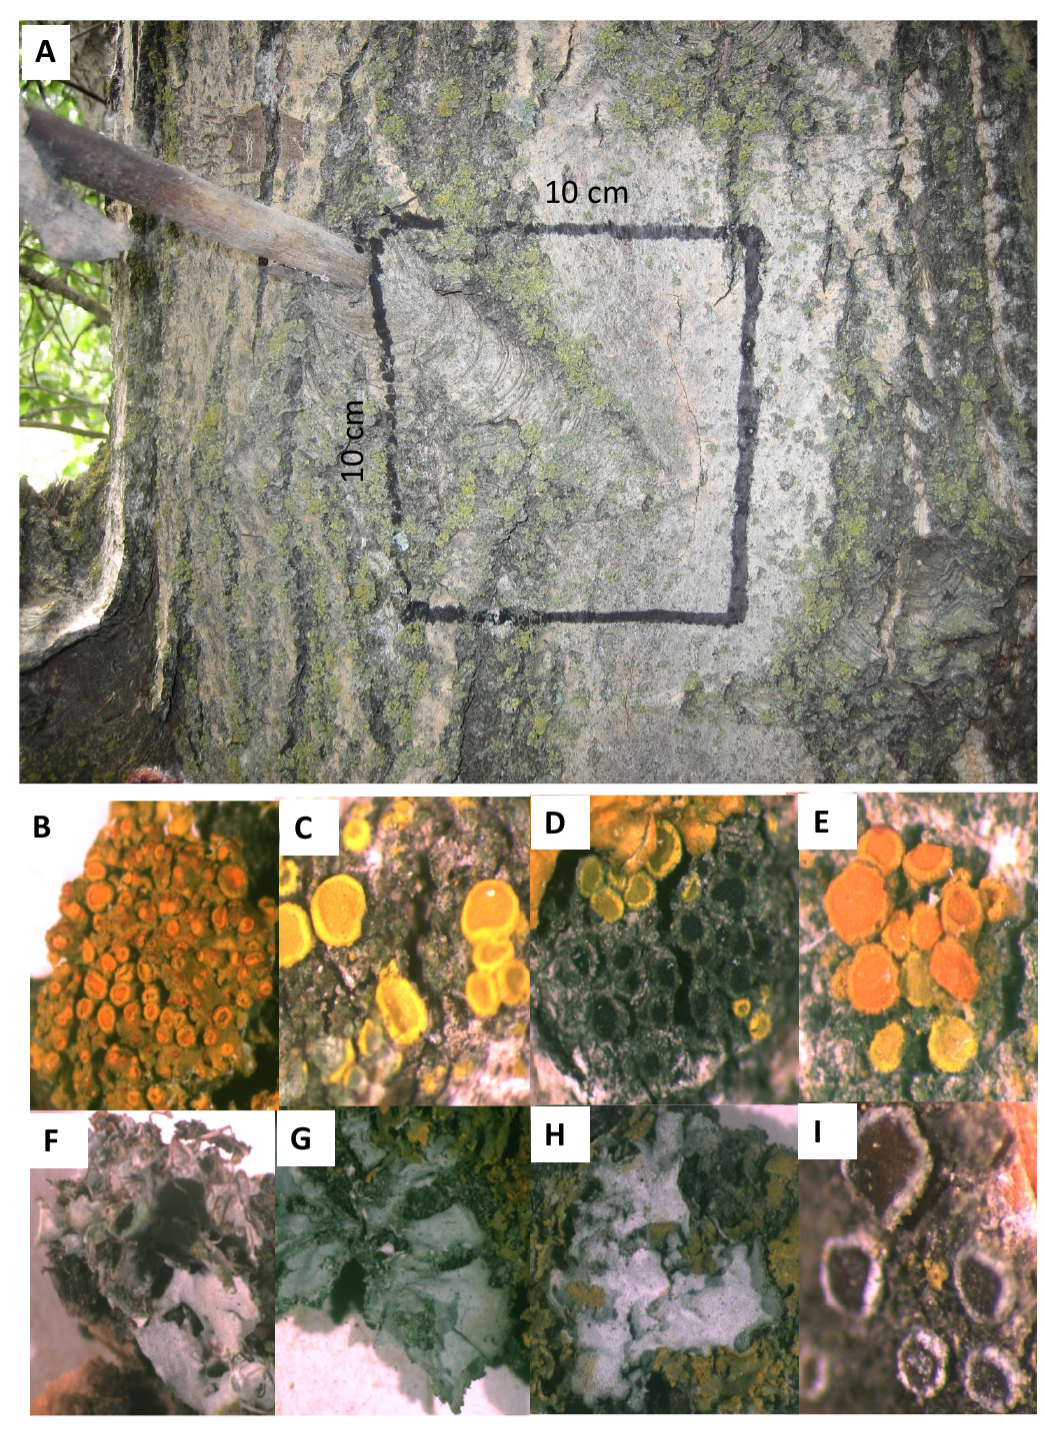
\includegraphics[width=\linewidth]{lcn_sampling.png}
\caption{The communities of bark lichens were observed in a common
  garden of replicated genotypes of narrowleaf cottonwood trees
  (\textit{P. angustifolia}) at the Ogden Nature Center (Ogden,
  UT). (A) Lichens were sampled within a fixed area (100 cm$^2$) on
  individual trees at two heights, 50cm and 95cm from the
  ground. (B-I) Close-up photos show the other lichen species
  observed, respectively:  \textit{X. montana}, \textit{Candelariella
    subdeflexa}, \textit{Rinodina} sp., \textit{Caloplaca holocarpa},
  \textit{Physcia adscendens}, \textit{Phyciella melanchra},
  \textit{Physcia undulata} and \textit{Lecanora hagenii}. Photo
  Credits: L.J. Lamit (B-D) and R.R. Naesbourg (E-I).}
\label{fig:lichen_sampling}
\end{figure}


\subsection*{Lichen Network Modeling and Analysis}

For each tree, repeated observations of lichen were made in order to
construct replicated interaction networks for each genotype. We
conducted a modified sampling procedure originally developed by
\citep{Lamit2015a} with the addition that we quantified the presence
of lichen in the 1 cm$^2$ cells on individual trees of
\textit{P. angustifolia}. Unipartite networks were generated using the
conditional probabilities of each species pair, i.e. the probability
of observing one species given an observation of another species
$P(S_i | S_j)$, based on the method developed by
\citep{Araujo2011}. To calculate conditional probabilities, we
quantified the individual probabilities of species occurrences
$P(S_i)$ and the joint probability of co-occurrences $P(S_i, S_j)$
using the frequencies of each species and their co-occurrences. We
were then able to calculate the conditional probabilities of each
species pair as $P(S_i|S_j) = \frac{P(S_i,S_j)}{P(S_j)}$, based on the
axioms of probability. This yielded a matrix that could possibly be
asymmetric, i.e. $P(S_i|S_j)$ does not have to be equal to
$P(S_j|S_i)$. Another important property of this matrix is that the
diagonal, $P(S_{i} | S_{i})$, was equal to one for all species present
and zero for species that were not observed in any cell.

We then applied an analytical procedure to remove non-significant
links between species. This procedure determines if the joint
probability of a species pair (i.e. $P(S_i,S_j)$) is different from
zero (Fig.~\ref{fig:conet_method}).  Here, a confidence interval
$CI_{95\%}$ is calculated as as $CI_{95\%} = E[S_iS_j] * Z_{95\%} *
\sqrt{V(S_iS_j)}$, where the expected frequency of co-occurrences
E($S_iS_j$) is the total number of cells surveyed ($N$) times the
independent probabilities of each species $P(S_i) * P(S_j)$,
$Z_{95\%}$ is the Z-score for 95\% from a Z-distribution and the
expected variance of $E(S_iS_j)$ is the total number of cells times
the expected probability of $S_iS_j$ and its compliment
(i.e. $V(S_iS_j) = N * E[P(S_i,S_j)] * (1 - E[P(S_i,S_j)])$). If the
observed number of co-occurrence falls outside of the confidence
interval, the joint probability $P(S_i,S_j)$ is determined to be equal
to the product of the individual probabilities (i.e. $P(S_i) \dot
P(S_j)$), and the conditional probability reduces to the individual
probability of that species $P(S_i)$. Therefore, unless the
co-occurrence of a species pair falls outside the confidence interval,
the probability that the observation of one species given the other is
no different than simply observing that species alone. This enables us
to remove links from a given network by re-scaling the resulting
conditional probabilities by subtracting the individual probabilities
from the conditional probabilities (i.e. how different the conditional
probability is from the independent probability), which makes any
species with a non-significant conditional probability zero. 

The resulting matrix ($\mathbf{D} = D_{ij}$) can be interpreted as one
species' impact on another with zero being no effect and values less
than or greater than zero being negative and positive effects,
respectively. Here, we will refer to $\mathbf{D}$ as a signed,
weighted interaction matrix. As such, $\mathbf{D}$ has the properties
that it can be asymmetric (i.e. $D_{ij}$ does not necessarily equal
$D_{ji}$) and it scales between -1 and 1, and, therefore, does not
have the mathematical properties of a probabilistic network
\cite{Poisot2015}. Also, as the method does not track individuals
within species and interactions such as competitive exclusion or
facilitation within species would result in the same species being
observed. Therefore, the results of intra-specific interactions always
results in the same species being observed and a resulting $D_{ii} =
0$.

\begin{figure*}[ht]
\centering
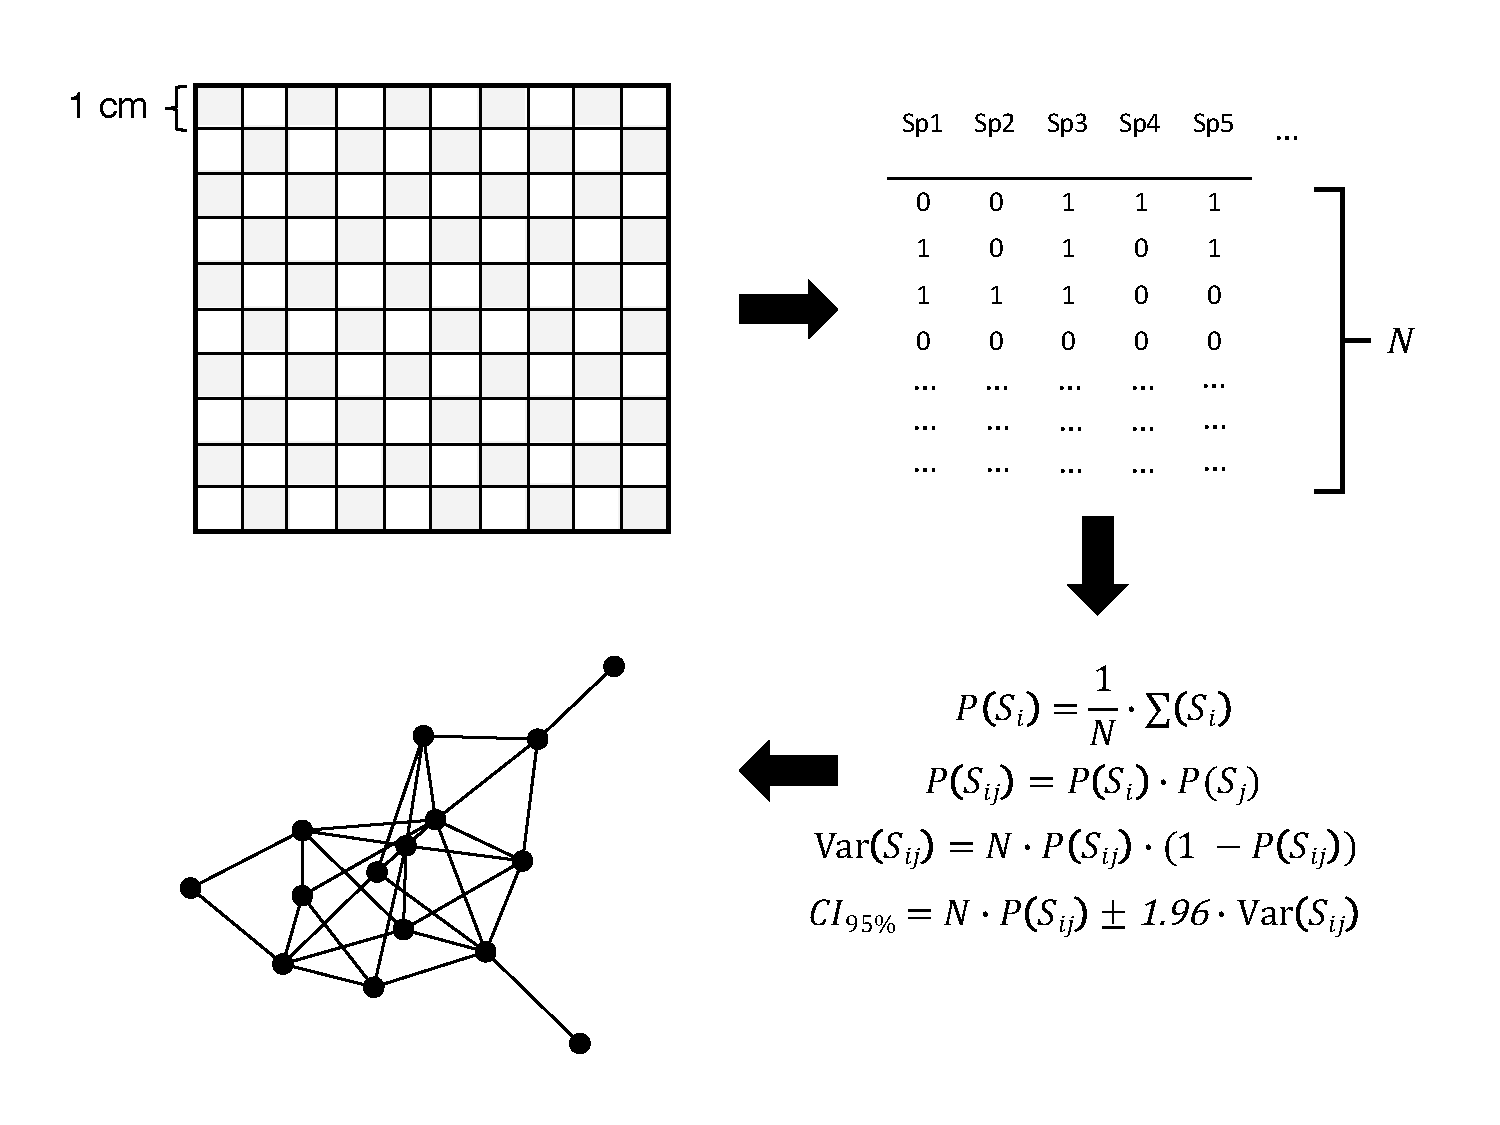
\includegraphics[width=\linewidth]{lcn_araujo_method.pdf}
\caption{Lichen interaction networks were constructed by conducting
  field observations in 1 cm$^2$ cells within a 100 cm$^2$ grid on each
  tree using a checkerboard pattern (grey cells). Thus, a set of $N$
  total cell observations were recorded for each tree with the
  presence or absence of each species recorded for each cell. Applying
  the probability-based network modeling method adapted from
  \cite{Araujo2011}, we calculated the conditional probabilities,
  $P(S_i|S_j)$, for all species pairs and removed (i.e. set equal to
  zero) species pairs whose joint probabilities, $P(S_i S_j)$, were
  not significant using a confidence interval based comparison of
  their observed co-occurrence frequency, $S_iS_j$, to that expected
  due to chance alone, $E[P(S_iS_j)] = P(S_i) P(S_j)$, and
  $P(S_i|S_j)$ reduces to $P(S_i)$, the observed individual
  probability of species $S_i$. In the context of these networks,
  asymmetry and positive/negative valued connections are distinct
  quantities. In-coming and out-going connections can be interpreted
  as ``influenced by'' and ``influenced'', respectively; while
  positive and negative should be seen as one species increasing or
  decreasing, respectively, the probability of another species'
  occurrence.}
\label{fig:conet_method}
\end{figure*}


\subsection*{Network Metrics}

To quantify the structural variation of lichen networks we calculated
several metrics at both the node and whole-network level. For
individual nodes (i.e. species) in each network, we calculated both
the degree and the Freeman's centrality \cite{sna}. We also calculated
two similar global network metrics: degree and centralization. The
first was network degree, which is a count of the total number of
links in a network. As the networks contained not only positive and
negative connections, as well as directional connections (both
in-coming and out-going), we calculated the same network metrics for
all combinations of these types of connections in each
network. Although there are many more possible network metrics that
could have been examined, we chose to focus on a restricted set for
the sake of clarity. Also, degree and centrality form the basis of
many other network metrics. To calculate separate metrics for positive
and negative links, we applied methods for calculating the centrality
accounting for the sign differences \cite{Everett2014NetworksTies}
using the \texttt{signnet} package \cite{siggnet}.


\subsection*{Statistical Analyses, Software and Data}

We used a combination of parametric and non-parametric, permutation
based frequentist statistical analyses to test for the effects of
genetic variation on lichen communities and their interaction
networks. To assess the effect of genotype on univariate responses, we
used additive, random effects models with Restricted Maximum
Likelihood (REML). We used a combination of Least Squares Regression,
Analysis of Variance (ANOVA) and correlation tests to quantify and
test for the relationship among other variables. Bark roughness,
lichen cover and species richness were square-root transformed to meet
the assumptions of homogeneity of variance and normality for these
tests.

For multivariate response variables, such as lichen community
composition and network structure, we used distance based multivariate
statistical approaches, including Permutational Analysis of Variance
(PERMANOVA) and Mantel tests. To quantify the similarity of lichen
networks among individual trees, we calculated the pairwise Euclidean
distance of the $\mathbf{D}$ interaction matrices among all pairs of
trees.

For visualization of multivariate patterns, we used Non-metric
Multi-Dimensional Scaling (NMDS) \cite{ecodist} to produce
dimensionally reduced ordinations of these multi-variate responses and
fitted vectors for continuous predictor variables to the ordinated
values \cite{vegan}. Using random initial configurations with a
maximum of 500 iterations and a change in stress threshold of less
than 10$^{-12}$. Final configurations has the lowest stress with at
most a stress level of 0.10.

For each network, we also calculated metrics that measure different
structural aspects. Although there are many other metrics, for the
sake of simplicity we focus on a subset that represent several
interesting features of network structure (see \citep{Lau2017a}). We
calculated the number of interactions or ``links'' in each network,
which provides a measure of the size of the network \citep{Lau2015a,
  Borrett2014EnaR:Analysis}. We also calculated the centralization of
each network, which measures the evenness of the distribution of
interactions among the species in the network \cite{sna}. In a network
with a low level of centralization species have similar amount of
interaction in the network, while a network with a high level of
centralization tends to have one or small number of species that
interact with other species. We used a related function to calculate
the centrality of each species (i.e. node level centrality) in each
network as well.

For all tests where genotype was used as a predictor, we quantified
the heritability of the response variable. Because the trees in the
garden were clonal replicates of each genotype, we calculated
broad-sense heritability, which is the genotypic variance divided by
the total phenotypic variance \cite{Conner2004ATextbook}. This can be
interpreted as a measure of the phenotypic variance due to genotypic
variation. We also apply this to the community genetics context as the
variance in \textit{extended} phenotypic variance due to genotypic
variation \cite{DawkinsTheGene}. For the multivariate analyses, where
we employ PERMANOVA, we followed the methods of
\citep{Shuster2006COMMUNITYSTRUCTURE} to adjust the degrees of freedom
for unbalanced genotype replicates.

All code and data for the project are openly available online. Code
and data are available at \url{github.com/ecgen/comgen}. The project
is also archived via Zenodo at \url{zenodo.com/doiXXXXXX}. All
analyses were conducted using the programming language R version 3.6.1
(R Development Core Team 2019).

\begin{figure}[ht]
\centering
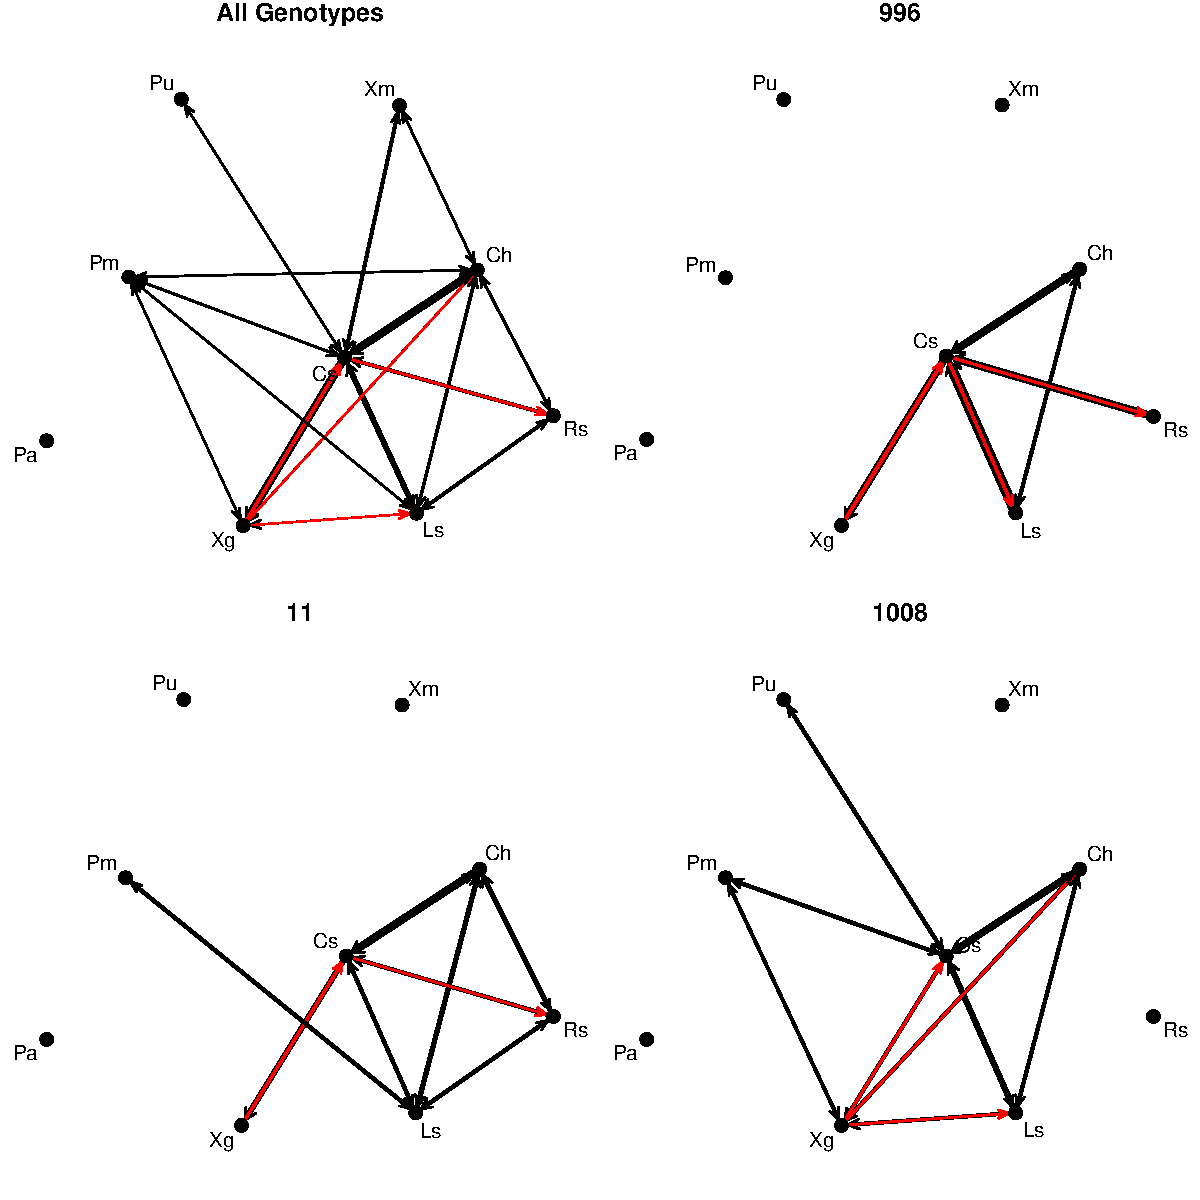
\includegraphics[width=\linewidth]{cn_onc.pdf}
\caption{Lichen networks varied in structure among tree
  genotypes. Network diagrams of the mean lichen interaction matrices
  averaged for all trees and for several individual genotypes (996,
  WC5 and 1008) showing a range of interaction network
  structure. Directionality (arrowheads) and sign (red = negative,
  black = positive) of interactions are shown as edges between species
  (abbreviated by the first letter of the genus and specific epithet),
  which are scaled by their magnitude. The sign of the interaction is
  indicative of greater (positive) or lesser (negative) paired
  occurrences than expected relative to the overall frequency of
  occurrence of each species. Ecologically, the links in the network
  are likely the product of multiple types of interactions
  (e.g. mutualism, parasitism, competition, facilitation) that could
  vary over both space and time.}
\label{fig:geno_nets}
\end{figure}
}

\showmatmethods{} % Display the Materials and Methods section

\section*{Results}

%% New results Fri May  1 19:00:26 EDT 2020

Tree genotype influenced lichen network structure and multiple lichen
network metrics were heritable.  Tree genotype significantly predicted
the structural similarity of lichen networks (PERMANOVA:
Pseudo-$F_{9,27}$ = 3.58, $H^2$ = 0.41, \textit{p-value} = 0.0537)
(Fig.~\ref{fig:h2_plot}).  Overall network level metrics responded
significantly to tree genotype (Table~\ref{tab:h2_net}), including
network degree (\textit{RLRT} = 3.52, $H^2$ = 0.32, \textit{p-value} =
0.0255) and centralization including both in-coming and out-going
links (\textit{RLRT} = 4.04, $H^2$ = 0.33, \textit{p-value} = 0.0184)
or when separated into in-coming only (\textit{RLRT} = 3.9852, $H^2$ =
0.3309, \textit{p-value} = 0.0190) or out-going only (\textit{RLRT} =
3.8615, $H^2$ = 0.3193, \textit{p-value} = 0.0205).  Metrics including
only positive links also showed a significant effect of tree genotype,
including positive degree (\textit{RLRT} = 3.6925, $H^2$ = 0.3242,
\textit{p-value} = 0.0229), positive in-going centralization
(\textit{RLRT} = 4.4812, $H^2$ = 0.3487, \textit{p-value} = 0.0142)
Metrics calculated with negative links were not significant, including
degree (negative) (\textit{RLRT} = 0.0327, $H^2$ = 0.0318,
\textit{p-value} = 0.3859) and both in-coming (negative)
(\textit{RLRT} = 0.3304, $H^2$ = 0.1057, \textit{p-value} = 0.2508)
and out-going centralization (negative) (\textit{RLRT} = 0.0862, $H^2$
= 0.0513, \textit{p-value} = 0.3446).

\begin{figure*}[ht]
\centering
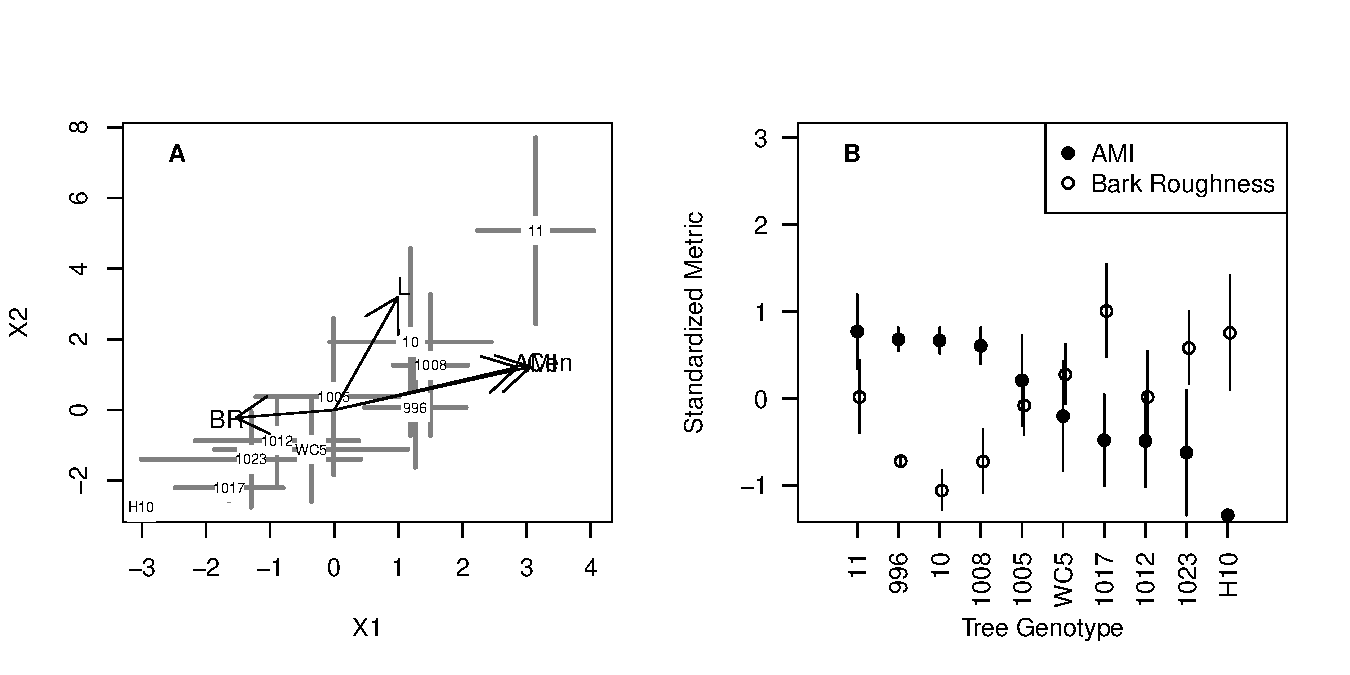
\includegraphics[width=\linewidth]{h2_plot.pdf}
\caption{The similarity of lichen networks varied among tree
  genotypes. A. The plot shows genotype centroids of NMDS ordinated
  (R$^2$ = 0.999, stress = 0.008) lichen network similarity ($\pm$ 1
  S.E.). Genotype centroids that are closer together tend to have more
  similar lichen network structure. Arrows showing the direction
  (arrowhead) and magnitude (length) of the vectors of correlation
  between bark roughness (\textbf{BR}) and network centralization
  (\textbf{Cen}) and the ordinated network similarity. B. Plot showing
  the standardized ($\frac{x - \bar{x}}{\sigma}$) means ($\pm$ 1 S.E.)
  for the two of the genetically based lichen network metrics: overall
  degree (i.e. total number of links) and centralization, which is a
  measure of the dominance of one species in the network.}
\label{fig:h2_plot}
\end{figure*}

% latex table generated in R 3.6.3 by xtable 1.8-4 package
% Thu May 14 16:39:05 2020
\begin{table}[ht]
\centering
\begin{tabular}{rrrr}
  \hline
response & statistic & H2 & p-value \\ 
  \hline
Lichen Network Similarity & 3.5821 & 0.4130 & 0.0537 \\ 
  Centralization & 4.0444 & 0.3305 & 0.0184 \\ 
  Centralization In-Degree & 4.4812 & 0.3487 & 0.0142 \\ 
  Centralization In-Degree (positive) & 3.9852 & 0.3309 & 0.0190 \\ 
  Centralization In-Degree (negative) & 0.3304 & 0.1057 & 0.2508 \\ 
  Centralization Out-Degree & 3.8615 & 0.3193 & 0.0205 \\ 
  Centralization Out-Degree (positive) & 3.5585 & 0.3119 & 0.0248 \\ 
  Centralization Out-Degree (negative) & 0.0862 & 0.0513 & 0.3446 \\ 
  Number of Network Links (Degree) & 3.5175 & 0.3156 & 0.0255 \\ 
  Degree (positive) & 3.6925 & 0.3242 & 0.0229 \\ 
  Degree (negative) & 0.0327 & 0.0318 & 0.3859 \\ 
   \hline
\end{tabular}
\caption{Genotypic effects on the associated lichen network structure.} 
\label{tab:h2_net}
\end{table}


The genetic response of network centralization was driven by variation
in \textit{Caloplaca holocarpa}. Centrality varied significantly among
species ($F_{8, 324}$ = 7.99, $R^2$ = 0.16, \textit{p-value} $<$
0.0001). \textit{Caloplaca holocarpa} centrality was the main species
to exhibit a significant response to tree genotype in terms of
positive centrality for both the in-coming (\textit{RLRT} = 3.61,
$H^2$ = 0.32, \textit{p-value} = 0.0240) and out-going (\textit{RLRT}
= 3.13, $H^2$ = 0.30, \textit{p-value} = 0.0327) perspectives, but not
for either negative centrality metrics in-coming (\textit{RLRT} = 0,
$H^2$ = 0, \textit{p-value} = 1) or out-going (\textit{RLRT} = 0,
$H^2$ = 0, \textit{p-value} = 0.4543). None of the other species'
centralities showed a genotypic response (Supplementary
Table~\ref{tab:sppcen}) with the exception of \textit{X. montana}
(\textit{RLRT} = 2.92, $H^2$ = 0.32, \textit{p-value} = 0.0375);
however, the centrality of \textit{X. montana} was much lower overall
relative to \textit{C. holocarpa} and the variation in
\textit{X. montana} centrality was restricted to two genotypes
(Fig.~\ref{fig:geno_sppcen}).



\begin{figure*}[ht]
\centering
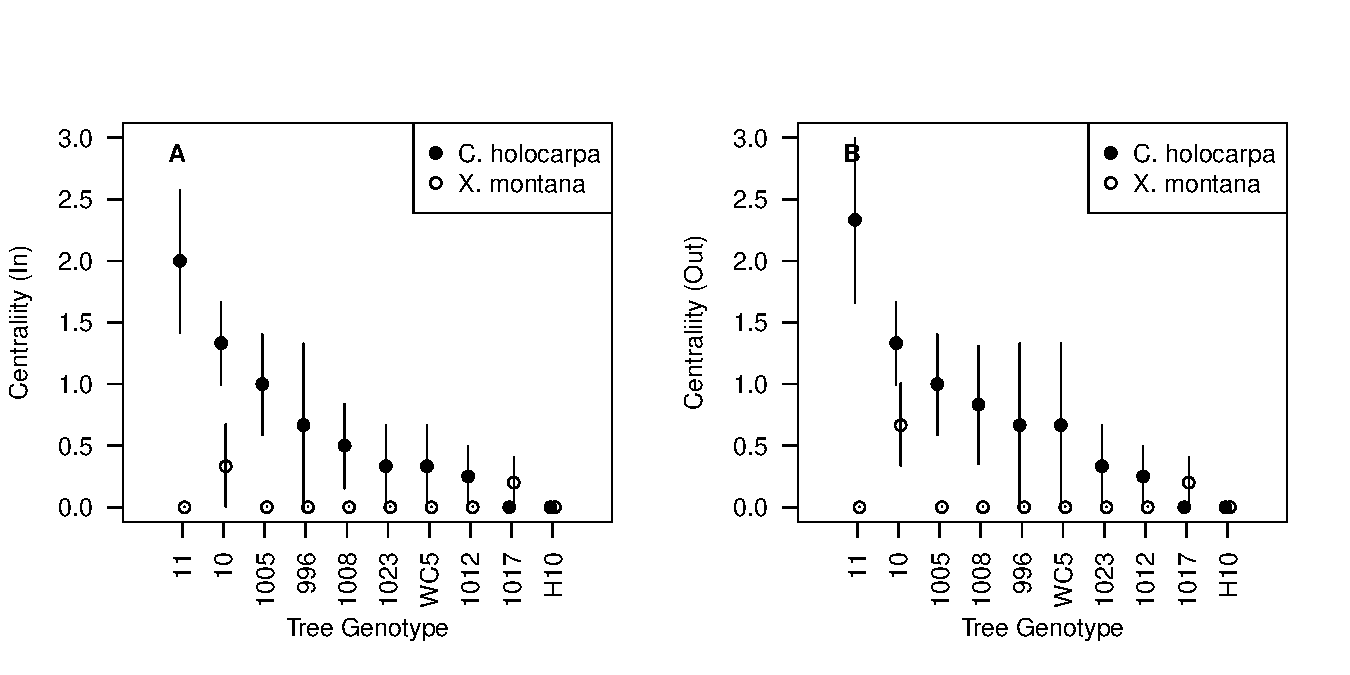
\includegraphics[width=\linewidth]{geno_sppcen.pdf}
\caption{Dot-plots showing the mean (dot) and $\pm$ 1 SE of in-degree
  (A) and out-degree (B) centrality for two species,
  \textit{C. holocarpa} and \textit{X. montana}. \textit{Caloplaca
    holocarpa} centrality was highly variable among
  genotypes. \textit{Xanthomendoza montana} centrality, both in- and
  out-degree, was only non-zero for two genotypes, and only out-degree
  centrality displayed a significant response to genotype.}
\label{fig:geno_sppcen}
\end{figure*}

\textit{Add transformations of variables to methods.}

Genotype indirectly influenced lichen network centralization via the
genetically based variation in bark roughness. The percent cover of
rough bark (\textit{RLRT} = 4.8526, $H^2$ = 0.3221, \textit{p-value} =
0.0113) and condensed tannins (\textit{RLRT} = 3.0522, $H^2$ = 0.3205,
\textit{p-value} = 0.0343) both displayed significant responses to
tree genotype. None of the other bark traits, pH (\textit{RLRT} =
0.00, $H^2$ = 0.00, \textit{p-value} = 1.0000) or carbon-nitrogen
ratio (\textit{RLRT} = 0.0000, $H^2$ = 0.0000, \textit{p-value} =
1.0000), showed a significant response to tree genotype and none other
than bark roughness was correlated with network similarity
(Table~\ref{tab:cn_trait_perm}); therefore, we focused our subsequent
analyses on the indirect effect of genotype on lichen network
structure via bark roughness. We found that bark roughness was
significantly correlated with network similarity (PERMANOVA:
Pseudo-$F_{1,32}$ = 13.029, $R^2$ = 0.26, \textit{p-value} = 0.0096)
and other lichen network metrics, including negative correlations with
overall network degree ($df$ = 35, $t$ = -2.13, $r$ = -0.34,
\textit{p-value} = 0.04) and centralization ($df$ = 35, $t$ = -2.52,
$r$ = -0.39, \textit{p-value} = 0.02). In other words, trees with more
similar levels of bark roughness tended to have lichen interaction
networks with similar structure. To quantify the genetic bases of this
effect of bark roughness on network structure, we used the residual
values from regressions of network degree and centralization in tests
of the effect of tree genotype and found no significant effect of tree
genotype for either degree (\textit{RLRT} = 0.00, $H^2$ = 0.00,
\textit{p-value} = 1.0000) or centralization (\textit{RLRT} = 0.00,
$H^2$ = 0.00, \textit{p-value} = 1.0000), suggesting that the observed
relationship between bark roughness and lichen network structure was
largely genetically based (Fig.~\ref{fig:br_net}).

% latex table generated in R 3.6.3 by xtable 1.8-4 package
% Thu May  7 18:13:05 2020
\begin{table}[ht]
\centering
\begin{tabular}{rrrrrr}
  \hline
 & Df & SumOfSqs & R2 & F & Pr($>$F) \\ 
  \hline
BR & 1.0000 & 21021.8765 & 0.2595 & 13.0299 & 0.0096 \\ 
  CT & 1.0000 & 2349.3142 & 0.0290 & 1.4562 & 0.2016 \\ 
  pH & 1.0000 & 2098.8999 & 0.0259 & 1.3010 & 0.2899 \\ 
  CN & 1.0000 & 3896.1757 & 0.0481 & 2.4150 & 0.1890 \\ 
  Residual & 32.0000 & 51627.3270 & 0.6374 &  &  \\ 
  Total & 36.0000 & 80993.5932 & 1.0000 &  &  \\ 
   \hline
\end{tabular}
\caption{PERMANOVA Pseudo-F Table of lichen network similarity response to bark traits.} 
\label{tab:cn_trait_perm}
\end{table}


\begin{figure*}[ht]
\centering
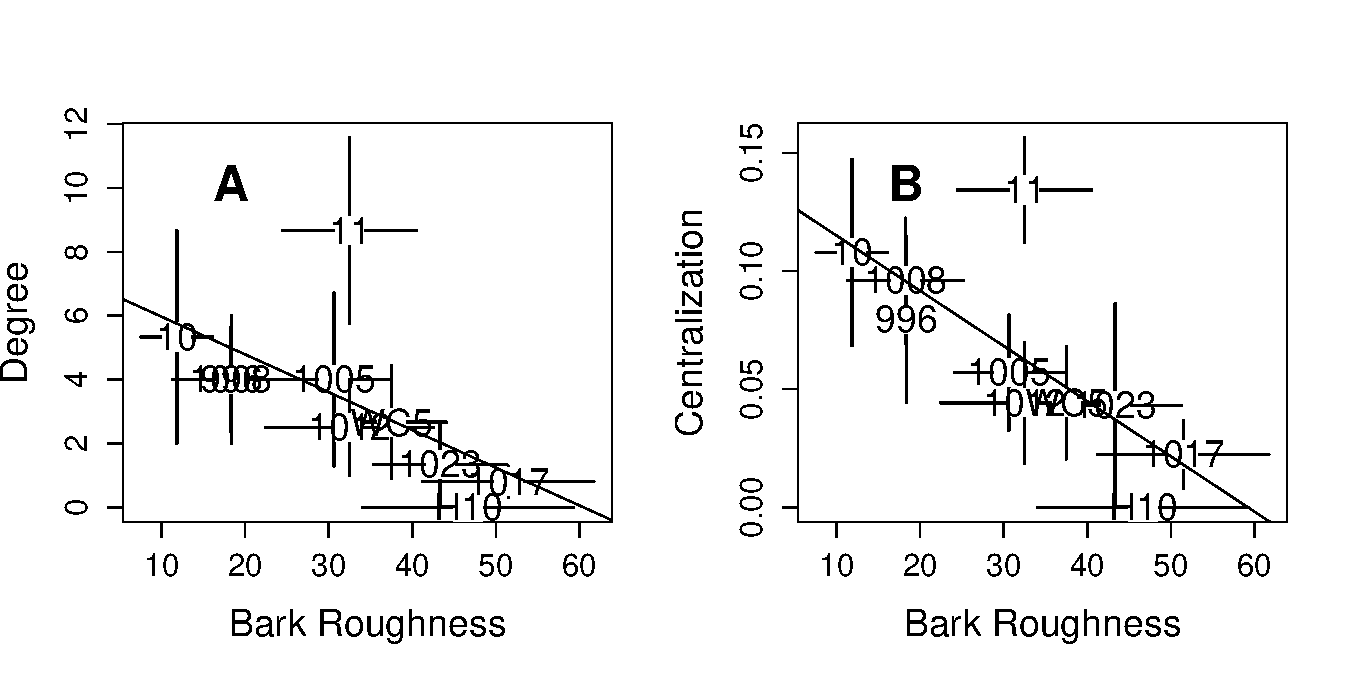
\includegraphics[width=\linewidth]{br_net.pdf}
\caption{Bivariate plots of the negative relationship between bark
  roughness and two network metrics: A) degree and B)
  centralization. Each plot displays the genotype mean ($\pm$ 1 S.E)
  for both variables and a least-squares regression line calculated
  using the genotype means. Generally, as roughness increased the
  number of interactions (degree) and dominance of
  those interactions decreased.}
\label{fig:br_net}
\end{figure*}


%% In addition to including your tables within this manuscript file, PNAS
%% requires that each table be uploaded to the submission separately as a
%% “Table” file.  Please ensure that each table .tex file contains a
%% preamble, the \verb|\begin{document}| command, and the
%% \verb|\end{document}| command. This is necessary so that the
%% submission system can convert each file to PDF.


\section*{Discussion}

The following is from Guimaraes 2020.

\begin{quote}
  The patterns of interaction in individual-based networks depart from
  these theoretical benchmarks, revealing the role of variability in
  space, time, traits, and preferences in shaping ecological
  interactions (Araújo et al. 2008).  Space and time create templates
  for ecological interactions (Cantor et al. 2018) that favor
  departures from homogeneous and abundance-based network
  patterns. The spatial configuration of an environment may foster the
  rise of modules of interacting individuals (Fortuna et al. 2009, Tur
  et al. 2015). Similarly, temporal variation in the availability of
  partners affects the network structure on different time scales
  (Dáttilo et al. 2014b, Valverde et al. 2016). For example, networks
  describing interactions among individual insects and different plant
  species show temporal modularity, with different individuals sharing
  pollen resources at different times in the flowering season (Tur et
  al. 2015). Space and time may therefore promote spatiotemporal
  variation in the network structure by affecting the likelihood of
  potential interactions. Even so, the macroscopic properties of
  individual-based networks may show structural constancy. For
  example, networks of interactions among protective ant species and
  individual plants show daily turnover in ant species, while
  maintaining nestedness and average levels of reciprocal
  specialization (Dáttilo et al. 2014b).  Space and time set the
  scales in which individual-based networks occur, but the interaction
  patterns are further modified by variation in individual traits. For
  example, the numbers of individual honeybees (Apis mellifera,
  Apidae) visiting thistle (Cirsium arvense, Asteraceae) flowers
  increase with the number of flower heads and the height of the
  inflorescences on individual plants (Dupont et al. 2011). Network
  description of intraspecific variation in dietary niches uncovers
  subtle associations between traits and resource use that go beyond
  the number of resources used.  For example, in a monomorphic
  population of three-spine sticklebacks (Gasterosteus aculeatus,
  Gasterosteidae), differences in trait combinations (e.g., body and
  snout shapes) were associated with dietary modules, i.e., groups of
  individuals feeding on similar prey (Araújo et al. 2008). Similarly,
  networks describing diet overlap among thick-billed murres (Uria
  lomvia, Alcidae) revealed sexbased dietary groups (Provencher et
  al. 2013). Network analyses can therefore reveal how patterns of
  interaction across individuals are associated with variation in
  individual traits.
\end{quote}

We found that tree genotype influenced lichen network structure in the
experimental cottonwood forest. Network similarity and metrics of
network structure tended to be more similar on trees of the same
genotype. Generally, this genetic effect was manifested in positive
interactions and largely driven by \textit{C. holocarpa}. The
genetically based trait, bark roughness, was the only trait observed
to effect network variation, largely via shifts in positive in-coming
and out-going interactions. Bark roughness has been demonstrated
previously to be under strong genetic control \cite{Bdeir2017}, and
bark roughness has also previously been shown to be an important tree
trait influencing bark lichens \cite{Lamit2015a}; however this is the
first demonstration of a link from genes to lichen network structure.
As such these results have important implications for the potential
influence of genetically based variation in ecosystems with networks
of interacting species.

\subsection*{Heritability of Interaction Network Structure}

We found significant heritability of lichen interaction network
structure, and, in line with the genetic similarity rule, networks
observed on trees of the same genotype tended to be structurally
similar. There are important functional ramifications of genetically
based variation in network structure. First, even if the composition
of the communities is the same among individuals and genotypes,
interactions may not be. We didn't observe compositional differences
using the same data from which the lichen networks were derived. If we
only had our composition dataset from this study, we would have
concluded no response of the lichen community to tree genotype, even
though the underlying interactions among lichen species does vary
among genotypes. Community composition of lichen has previously been
observed to be different among tree genotype in the same experimental
garden, though this was observed with a larger sampling of total area
and quadrats per tree. Regardless, this could result in a situation
in which abundance based investigations of community-level genetic
effects may miss important variation in the interactions among
individuals in these communities, leading to an underestimate of
genetic effects in ecosystems. It is possible that these underlying
differences in interactions among lichen could lead to differences in
community composition at a future point in time, however, this is not
needed for evolutionary dynamics to play out.

Second, following on the previous point, genetic diversity could be
influencing the stability of communities through the effects on the
structure of interactions. Some network structures are likely to be
more stable, either in response to disturbance or via self-organized
dynamics. For example, centralized networks, although more efficient,
are theorized to be more susceptible to targeted attacks on the center
of the network. For example, consider a forest with two genotypes that
support lichen communities that are similar in total abundances of
each species but differ in terms of the structure. Extensions of game
theory to evolutionary biology have demonstrated that network
structure can lead to variation in evolutionary dynamics. Some
structures tend toward dominance and dampening of selection, while
others lead to amplification of selection (Newman). One class of
networks that are theorized to have amplifying effects on networks
have "star" shapes with one or a few species at the center and
radiating interactions out from the central core (Leiberman). This is
structurally what we have observed with the networks that tend to
occur on some of the genotypes in our study, i.e. the more centralized
networks. It is possible that these more centralized networks could
function as hot-spots of evolutionary dynamics resulting from the
amplifying effect the network structure fostered on that tree
genotype.



\subsection*{Implications for Interspecific Indirect Genetic Effects (IIGEs)}

Interspecific indirect genetic effects (IIGE) theory provides a
quantitative framework within which to approach evolutionary theory at
higher levels of biological organization: from populations to
communities and ecosystems. To date, this theory has focused on
modeling the strong effects of foundation species
\cite{Shuster2006COMMUNITYSTRUCTURE, Whitham2012}, but it has not yet
integrated developments in the ecological or evolutionary network
theory literature. This is to say that it has not developed a way to
examine complex interactions among species; however, previous studies
have demonstrated this network context is likely to be important, as
altering the structure of interaction networks provides a means for
genetic effects to be dampened or magnified within the system of
interacting species. For example, \citep{Keith2017} showed that the
genetics based interactions of aphid resistant and aphid susceptible
trees resulted in different interaction networks of their associated
arthropod communities composed of 139 species. At the scale of
ecosystems, trophic networks or food webs direct and control the rates
of energy and nutrient flux \cite{Borgatti2006}. Furthermore, in a
predator-prey-plant study, Smith \cite{Smith2011}, showed that the
interactions among species across trophic levels depended on plant
genotype. Also, work by \citep{Toju2017, Toju2016, Toju2014a} observed
consistent patterns of centralized interactions of species modules
focused around hubs of plant-fungal interactions. In other words, a
small number of plant and fungal symbionts tended to have
disproportionate numbers of interactions with other species and likely
are the drivers in determining community assembly, structure and
dynamics.

The results of the current study provides clear empirical evidence that
variation in network structure can be genetically based
(i.e. heritable) and points to the need to expand IIGEs encompass the
structure of interaction networks. Although such a synthesis
necessitates a much greater effort than can be afforded in this paper,
it is possible to point to several productive pathways forward. In
terms of interaction networks, foundation species are relatively
central within the system of interactions, that is their direct and/or
indirect effects are greater then other species. So, when the more
centralized (foundation) species have genetically based interactions,
genetic effects will tend to be magnified in the community. Here, we
found that even though more abundant or more centralized
(i.e. ``important'') species were present in the community, their
effects were not the main component responding to genetic
effects. Considering the impact of network structure would be a
productive path forward for the theoretical development and
application of the IIGE concept.


\subsection*{Evolutionary Implications of a Genetic Basis to Network Structure}

With regard to the evolutionary implications of network structure,
ecological network studies have focused on asymmetry and the
quantification of its structure in communities, with qualitative
discussion of the impacts on evolutionary dynamics
\cite{Bascompte2006, Diaz-Castelazo2010, Guimaraes2011,
  Thompson2013}. More specific predications, with a quantitative
framework, can be found in applications of evolutionary game theory,
and although developed at the population scale, such theory can apply
to communities. One seemingly useful direction from evolutionary
network developments from game theory is the classification of
networks into two general categories, rooted and cyclic, in which
rooted networks have interactions in which evolutionary effects
emanate from one or multiple origins but these effects do not have
connections back to the origins, whereas cyclic networks contain
feedbacks to one or more origins. Although it did not explicitly
define it in this context, the previous work of \citep{Lau2017a}
developed the perspective that the structure of the network in the
context of a foundation species, such as cottonwoods in which there
are demonstrable community level genetic effects, is inherently
created when trait variation among genotypes of a foundation species
has ecological effects on associated species. 

This builds on many previous studies demonstrating that the community
level effects vary among multiple genotypes. It is not clear what
potential there is for feedbacks there are to the origins (e.g. the
cottonwood genotypes) from the community, and as such it cannot be
determined whether these networks are cyclic or rooted. In other
systems, lignicolous lichens can have demonstrable positive effects on
the availability of nutrients for the trees that they are associated
with, but this has not been measured in the current
system. % MKL - Add more context of lichen effects on other species 
% including associated symbionts and the foundation species itself.
Elucidating the absence and/or presence and quantifying such
feedbacks would allow for the determination of the cyclic nature and
potential evolutionary dynamics of this system. The presence of
feedbacks would provide the potential for non-linear dynamics in which
evolutionary effects are dampened or amplified by the structure of the
network. For example, a star structure in which there is a primary or
core set of central species with feedbacks from the radiating species
has been demonstrated to be a structure that amplifies evolutionary
dynamics \cite{Lieberman2005EvolutionaryGraphs}. If such feedbacks do
not exist, and these sub-networks of the lichen and tree genotypes are
likely to be multi-rooted networks. Such a structure is theorized to
generally promote diversification as variation arising from the
shifting distribution of the ``roots'', i.e. genotypes; however, loss
of genotype/root diversity could lead to fixation of a single genotype
in the population and a decrease in community-wide diversity.

\subsection*{Applicability to Other Systems}

Although our study was conducted with a community of lichens, these
results can be generalized to other groups of diverse organisms around
the world that also exhibit significant genetic signals at the
community level \cite{Rowntree2011, Whitham2012}. However, there are
important points to consider when extending the observed genetically
based response of the lichen networks to other systems. As bark lichen
individuals do not move, but grow in a primarily two dimensional
plane, these communities and their interactions occur in the highly
localized context of the tree's bark surface. Lichen individuals are
also many orders of magnitude smaller than the tree individual in this
system \cite{Lamit2011}. For these reasons, the genetic effects on
these communities is not dampened by the movement of individuals and
the mixing of the effect of different tree genotypes on the lichen
community, as might occur for more mobile species (e.g. insects and
birds). Relatedly, we only examined lichen in this study, and other
species whose distributions, abundances and/or interactions vary in
their response to tree genotype, such as animals that may also impact
lichen communities, could be playing a role that we did not
examine. For example, an analysis of the multivariate correlations of
different components of the community in this system demonstrated
significant patterns of genetic co-responses to tree genotype,
supporting the non-mutually exclusive possibilities of shared
responses to tree genotype or tree genotypic effects on interactions
among these sub-communities \cite{Lamit2015c}. As such, although we
can not rule out the possibility that other unmeasured tree traits or
organisms correlated with bark roughness are underlying the observed
patterns, substantial research supports the importance of genetically
based tree traits for communities and ecosystems
\cite{DesRoches2018TheVariation}, and in particular bark roughness for
bark lichen communities \cite{Bdeir2017, Lamit2011, Lamit2015a}.

One final point to discuss is that in the present study lichen cover,
species richness and composition were not significantly responsive to
tree genotype, unlike what has been previously observed for lichen
\cite{Lamit2015a} and multiple taxa in this and other systems
\cite{DesRoches2018TheVariation}. This is likely the result of
differences in sampling method and the choice of genotypes leading to
overall higher abundances of observed lichens to assure the
possibility of observing lichen interactions. In the current study
mean percent total lichen cover among genotypes ranges from ~60-93\%
cover; whereas the range reported in \citep{Lamit2015a} is
0.86-18.73\%.  The previous study used a visual estimation method,
unlike the current study, which observed lichen at the scale of 1
cm$^2$ cells, which could over-estimate cover depending on the
frequency at which actual thallus size was less than 1 cm$^2$.  The
previous study used samples from both the northern and southern
aspects of each tree; whereas, the current study only observed lichen
on the northern aspect.  Also, our current results are likely
different from the previous study because the current study selected
genotypes that tended to have bark lichen, with the interest of
focusing on generating networks for comparison. These differences do
not negate the findings of either study but is important to explain
the differences in the findings, particularly in the community-level
effects of tree genotype and the general applicability to future
studies.


In attempting to apply these findings to other systems, it is
important to consider the spatial and temporal scaling of genetic
effects. In the present study, the sessile nature of lichens means
that individuals, and potentially multiple generations, live their
entire lives on a single tree. As such, our study examines one scaling
of a genetic effect, in which the phenotype of a single tree
individual (i.e., tree genotype) has complete influence on the
community with little to no effect of other tree individuals in the
population. The extreme from this would be where the associated
community moved among and interacted with not only other community
members but also multiple tree individuals at a high rate, as would be
the case with free-living animals (e.g. flying insects). In the latter
case, the effect of tree genetics would then be the integral effect of
all the tree individuals in the population, and, all other factors
being equal, any one tree genotype would have a lower effect on
associated community. In reality, ecosystems are a mixture of species
of different body sizes and life-histories, and, as such, vary in the
degree to which they interact with other organisms, which is the basis
of the theory of the geographic mosaic of co-evolution
\cite{Thompson2013, Thompson2013a}. It is now important to consider
how the impacts of genetic effects on the network structure of
sub-groups, such as lichens, may or may not propagate through the
ecosystem to more mobile organisms. As developed previously, the
degree to which a genetic effect influences the community is a
function of the fidelity of the genetic effect (i.e., heritability)
and both the frequency and the intensity of the interaction
\cite{Shuster2006COMMUNITYSTRUCTURE}. One possible path forward is for
future work to extend the many previous community genetics studies
that have focused on sessile organisms, such as galling insects
\cite{Bailey2005ImportanceInteractions, Whitham2006a, Crutsinger2014,
  Solance2015, Keith2017}, to quantify the frequency of these
interactions in the context of the larger community. This would
provide an estimate of the relative impact of these focal, often
termed foundation, species. In addition, community genetics theory has
only considered first order interactions, i.e., between two organisms
\cite{Shuster2006COMMUNITYSTRUCTURE, Whitham2012,
  Whitham2020IntraspecificEvolution}. Given that network structure
could be influenced by genetic effects, as evidenced by the present
study, assessing higher order interactions could provide a path
forward for theoretical advances that could help with identifying
important characteristics of sub-groups to focus on in empirical
studies.

%% The results of the current study also provide evidence for a mechanism
%% of the ``extended phenotype'' through the self-organization of
%% communities via network structure. %%% REVIEW ASCENDENCY
%% Genetics impacting interactions shifts abundances
%% Genetics impacting the structure of interaction networks creates feedbacks

\subsection*{Conclusion}

In the face of the high degree of complexity and potential context
dependency of ecological processes, the current study points to the
utility of considering the spatial and temporal scales of
interactions, as discussed to some in previous studies
\cite{Bangert2006, Zook2010, Zytynska2012}. In the present study, we
found that community assembly processes, such as environmental
filtering and species interactions, are genetically based. This is
likely due, in part, to the large difference in the differences in
size and longevity of the lichen and cottonwood individuals with the
trees determining the environment in which the lichen occur. We
suggest that future work would be aided by determining these modules
within the biotic community that include species with similar
differences in body-size and time-scales. As heritable variation is
the raw material for natural selection to act upon, a genetic basis
for interaction network structure indicates evolutionary dynamics
should be considered at the community level and that conserving
genetic variation is important to consider in efforts to restore or
preserve complex species interactions and their associated ecosystem
functions \cite{Evans2013}.  With such findings, it appears that we
are closer to understanding the evolutionary drivers of Darwin's
entangled bank and the interconnectedness of species in complex
communities.





%% \textbf{TGW:  Is there any adaptive component to the tree in having
%%   certain lichen communities?  e.g., can they feed back to affect tree
%%   performance in some way or is this a passive outcome of a trait that
%%   affects bark for other adaptive reasons and lichens are passive
%%   players that tag along for the ride?  I could envision that lichens
%%   covering the bark of a tree act as a barrier between insects and
%%   pathogens, much like ectomycorrhizae cover fine roots as a first
%%   line of defense by invading microorganisms.  Uptake of N that gets
%%   passed to the tree??}


%% \textbf{LJL: I agree that there is a general overarching theme that
%%   evolution occurs in a community network context, but I’m not sure
%%   that we should state that as our main hypothesis. It seems more that
%%   this is a fundamental foundation for our work. The hypothesis is
%%   more what we are testing directly, but we don’t test this
%%   directly. I guess I don’t want to give the impresison that our
%%   communities are necessarily the result of each species evolving into
%%   its place in the community on these tree genotypes (although I do
%%   understand this as Shuster et al 2006’s fundamental explanation for
%%   why we see different communities on different genotypes; I don’t
%%   necessarily agree that this is the only reason we woudl see
%%   different communities on dif genotypes). Most of these are pretty
%%   generalist lichens, which could be found on other decidous trees in
%%   the surounding city or natural areas. I would look at it more like
%%   an assembling of lichen species into unique configurations on
%%   genetically different substrates. There may be some selection for
%%   different genotype of lichen during the community assembly process
%%   but we can’t really tell that just by differences in species
%%   abundances or coocurneces. I guess to me the evolutionary context
%%   that is more direclty related to this work is that the tree genotype
%%   is a central controller (indeed a sort of hub species in the
%%   network) of network structure. By anchoring the lichen network to
%%   tree genotype (and variation among networks to variation among tree
%%   genotypes) , our study highlights the possibility that natural
%%   selection acting on the trees may have an extended consequence for
%%   the network structure of organisms living on the trees…the extra
%%   thing we add to the field is that we show interaction networks are
%%   sensitive to genotype. I doubt the lichens have a direct effect on
%%   tree fitness, but favorability of some tree genotypes over others
%%   during natural selection will then go on to favor and disfavor
%%   certain lichen communities of different network structures. By being
%%   sensitive to tree genotype, the lichen community networks are
%%   passive riders on the waves of evolutionary dynamics that occur
%%   within the tree species they inhabit.}

%% \textbf{TGW: might be good to \cite papers on competition in lichens or
%%   other organizing factors to back up the least expected statement.
%%   as epiphytes we might not expect them to care.}

%% \textbf{TGW: I think we need to emphasize the long-term nature of our
%%   common garden study as very few common garden studies of lichens
%%   likely exist. Any refs on this? If true might want to mention this
%%   up front in intro.}

%% \textbf{MKL: Environmental filtering is evidenced by species richness,
%%   but also possibly species interaction varying based on environment
%%   as networks varied in terms of sign and magnitude as well.}

%% \textbf{MKL: The effect of bark roughness on network similarity was
%%   primarily genetically based, and there are likely other factors at
%%   play.}

%% \textbf{Discussion of network implications for stability with genetics.}


%% Please include your acknowledgments here, set in a single
%% paragraph. Please do not include any acknowledgments in the
%% Supporting Information, or anywhere else in the manuscript.



\acknow{This work was supported by the National Science Foundation grant
(DEB-0425908) and Integrative Graduate Research Traineeship (IGERT)
fellowships for M.L. and L.L. The Ogden Nature Center staff helped to
maintain the common gardens. Lichen sampling was supported by Todd
Wojtowicz, Luke Evans and David Solance Smith.}

\showacknow{} % Display the acknowledgments section

\bibliography{lichen_network_genetics, r_pkgs}

\newpage
\section*{Supplementary Materials}

\setcounter{figure}{0}
\setcounter{table}{0}

\subsection*{Tables}

\newpage
% latex table generated in R 4.0.2 by xtable 1.8-4 package
% Mon Feb  1 16:21:36 2021
\begin{table}[ht]
\centering
\begin{tabular}{rrrrrr}
  \hline
 & df & SS & R2 & F & p-value \\ 
  \hline
geno & 9.00 & 44078.13 & 0.54 & 3.58 & 0.05 \\ 
  Residual & 27.00 & 36915.46 & 0.46 &  &  \\ 
  Total & 36.00 & 80993.59 & 1.00 &  &  \\ 
   \hline
\end{tabular}
\caption{PERMANOVA Pseudo-F Table of lichen network similarity to genotype.} 
\label{tab:cn_perm}
\end{table}


\newpage
% latex table generated in R 3.6.3 by xtable 1.8-4 package
% Tue May  5 16:04:30 2020
\begin{table}[ht]
\centering
\begin{tabular}{lll}
  \hline
Response & H2 & p-value \\ 
  \hline
Lichen Network Similarity & 0.413 & 0.0537 \\ 
  Average Mutual Information & 0.3101 & 0.0274 \\ 
  Network Centrality & 0.3305 & 0.0196 \\ 
  Number of Network Links & 0.3156 & 0.0269 \\ 
  Percent Lichen Cover & 0 & 1 \\ 
  Lichen Species Diversity & 0 & 0.4558 \\ 
  Lichen Species Richness & 0 & 0.458 \\ 
  Lichen Species Evenness & 0 & 1 \\ 
  Percent Rough Bark & 0.3221 & 0.0128 \\ 
  pH & 0 & 1 \\ 
  Carbon-Nitrogen (CN) Ratio & 0 & 1 \\ 
  Condensed Tannins (CT) & 0.0041 & 0.4513 \\ 
  BR-L Residuals & 0 & 1 \\ 
  BR-Cen Residuals & 0.0113 & 0.4357 \\ 
  BR-AMI Residuals & 0 & 1 \\ 
   \hline
\end{tabular}
\caption{Genotypic effects on the associated lichen community.} 
\label{tab:h2_table}
\end{table}



\newpage
% latex table generated in R 3.6.3 by xtable 1.8-4 package
% Tue May 12 16:32:48 2020
\begin{table}[ht]
\centering
\begin{tabular}{lllll}
  \hline
lichen species & mean & statistic & H2 & p-value \\ 
  \hline
Positive &  &  &  &  \\ 
  In-Degree &  &  &  &  \\ 
  X. galericulata & 0.2703 & 0 & 0 & 1 \\ 
  C. subdeflexa & 0.8919 & 2.1926 & 0.2158 & 0.0595 \\ 
  L. spp. & 0.4324 & 0 & 0 & 1 \\ 
  C. holocarpa & 0.5946 & 3.6146 & 0.3241 & 0.024 \\ 
  X. montana & 0.0541 & 0 & 0 & 0.4543 \\ 
  P. melanchra & 0.1351 & 0 & 0 & 1 \\ 
  P. adscendens & 0 &  &  &  \\ 
  P. undulata & 0.027 & 0 & 0 & 0.4543 \\ 
  R. sp. & 0.1351 & 2.049 & 0.2613 & 0.0656 \\ 
  Out-Degree &  &  &  &  \\ 
  X. galericulata & 0.027 & 0 & 0 & 0.4543 \\ 
  C. subdeflexa & 0.6757 & 0 & 0 & 1 \\ 
  L. spp. & 0.5946 & 0.0061 & 0.0126 & 0.4246 \\ 
  C. holocarpa & 0.7027 & 3.1318 & 0.2981 & 0.0327 \\ 
  X. montana & 0.0811 & 2.9228 & 0.3163 & 0.0375 \\ 
  P. melanchra & 0.1351 & 0 & 0 & 1 \\ 
  P. adscendens & 0 &  &  &  \\ 
  P. undulata & 0.027 & 0 & 0 & 0.4543 \\ 
  R. sp. & 0.2973 & 0.1505 & 0.0612 & 0.3119 \\ 
  Negative &  &  &  &  \\ 
  In-Degree &  &  &  &  \\ 
  X. galericulata & 0 &  &  &  \\ 
  C. subdeflexa & 0.1892 & 0 & 0 & 0.4543 \\ 
  L. spp. & 0.1892 & 0.0015 & 0.0057 & 0.4398 \\ 
  C. holocarpa & 0.1351 & 0 & 0 & 1 \\ 
  X. montana & 0.027 & 0.0377 & 0.0394 & 0.3807 \\ 
  P. melanchra & 0 &  &  &  \\ 
  P. adscendens & 0 &  &  &  \\ 
  P. undulata & 0 &  &  &  \\ 
  R. sp. & 0.1622 & 0 & 0 & 1 \\ 
  Out-Degree &  &  &  &  \\ 
  X. galericulata & 0.2432 & 0 & 0 & 1 \\ 
  C. subdeflexa & 0.4054 & 0 & 0 & 0.4543 \\ 
  L. spp. & 0.027 & 0 & 0 & 0.4543 \\ 
  C. holocarpa & 0.027 & 0 & 0 & 0.4543 \\ 
  X. montana & 0 &  &  &  \\ 
  P. melanchra & 0 &  &  &  \\ 
  P. adscendens & 0 &  &  &  \\ 
  P. undulata & 0 &  &  &  \\ 
  R. sp. & 0 &  &  &  \\ 
   \hline
\end{tabular}
\end{table}


\newpage
% latex table generated in R 3.6.3 by xtable 1.8-4 package
% Wed Aug  5 18:51:05 2020
\begin{table}[ht]
\centering
\begin{tabular}{rrrrrrrrrrr}
  \hline
 & BR & CT & pH & CN & PC & SR & SE & SD & L & Cen \\ 
  \hline
BR &  &  &  &  &  &  &  &  & -0.34 & -0.39 \\ 
  CT &  &  &  & -0.34 &  &  &  &  & 0.34 &  \\ 
  pH &  &  &  &  &  &  &  &  &  &  \\ 
  CN &  &  &  &  &  &  &  &  &  &  \\ 
  PC &  &  &  &  &  & 0.49 &  &  &  & -0.46 \\ 
  SR &  &  &  &  &  &  &  & 0.76 & 0.47 &  \\ 
  SE &  &  &  &  &  &  &  & 0.85 & 0.45 &  \\ 
  SD &  &  &  &  &  &  &  &  & 0.59 & 0.33 \\ 
  L &  &  &  &  &  &  &  &  &  & 0.88 \\ 
  Cen &  &  &  &  &  &  &  &  &  &  \\ 
   \hline
\end{tabular}
\caption{Matrix of correlations among tree traits, lichen community metrics and network metrics} 
\label{tab:cormat}
\end{table}


\newpage
% latex table generated in R 3.6.3 by xtable 1.8-4 package
% Fri May  8 12:58:43 2020
\begin{table}[ht]
\centering
\begin{tabular}{lrrrrr}
  \hline
 & Df & SumOfSqs & R2 & F & Pr($>$F) \\ 
  \hline
geno & 9.0000 & 1.5049 & 0.2001 & 0.7507 & 0.8878 \\ 
  Residual & 27.0000 & 6.0143 & 0.7999 &  &  \\ 
  Total & 36.0000 & 7.5193 & 1.0000 &  &  \\ 
   \hline
\end{tabular}
\caption{Pseudo-F Table of lichen community similarity PERMANOVA.} 
\label{tab:com_perm}
\end{table}


\newpage
\subsection*{Figures}

\begin{figure*}[ht]
\centering
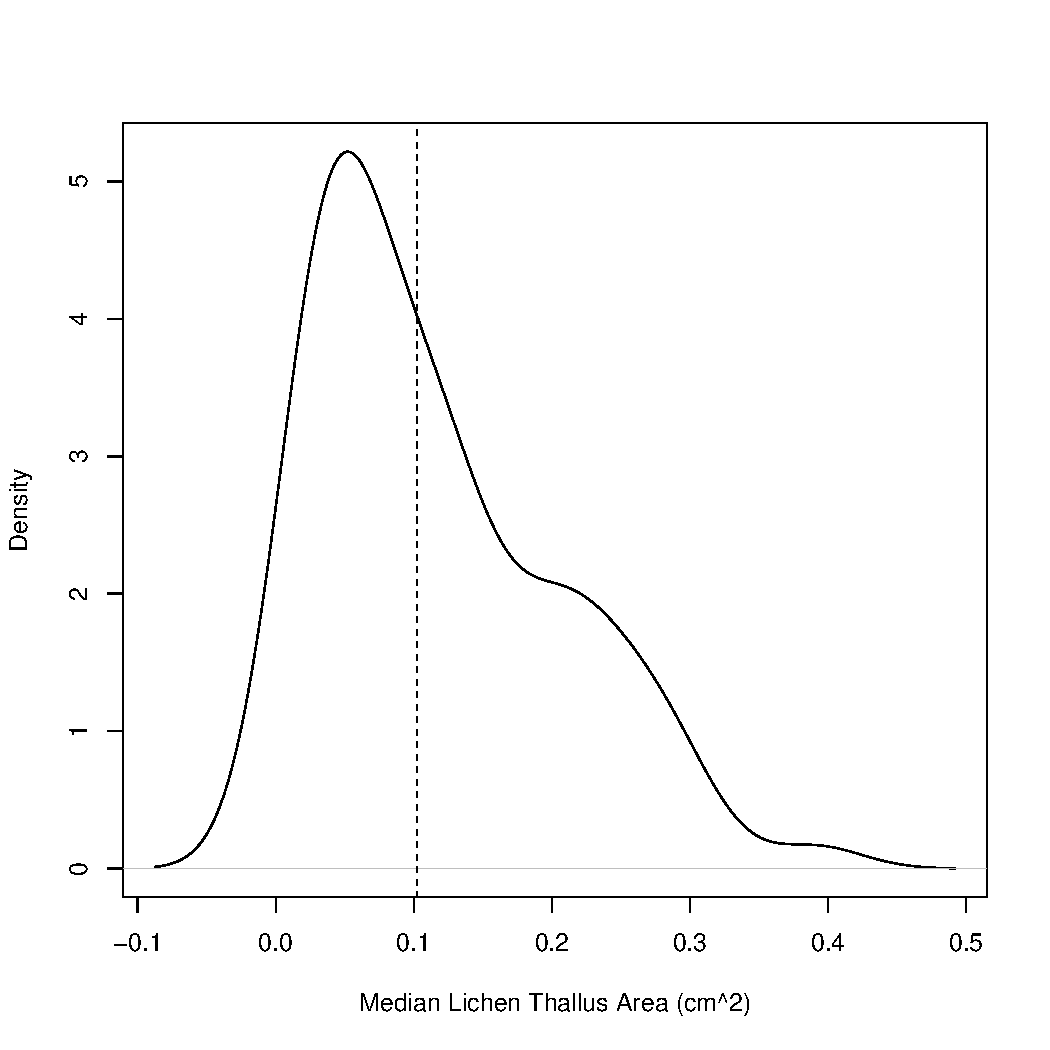
\includegraphics[width=\linewidth]{xg_size.pdf}
\caption{}
\label{fig:xg_size_app}
\end{figure*}

\begin{figure*}[ht]
\centering
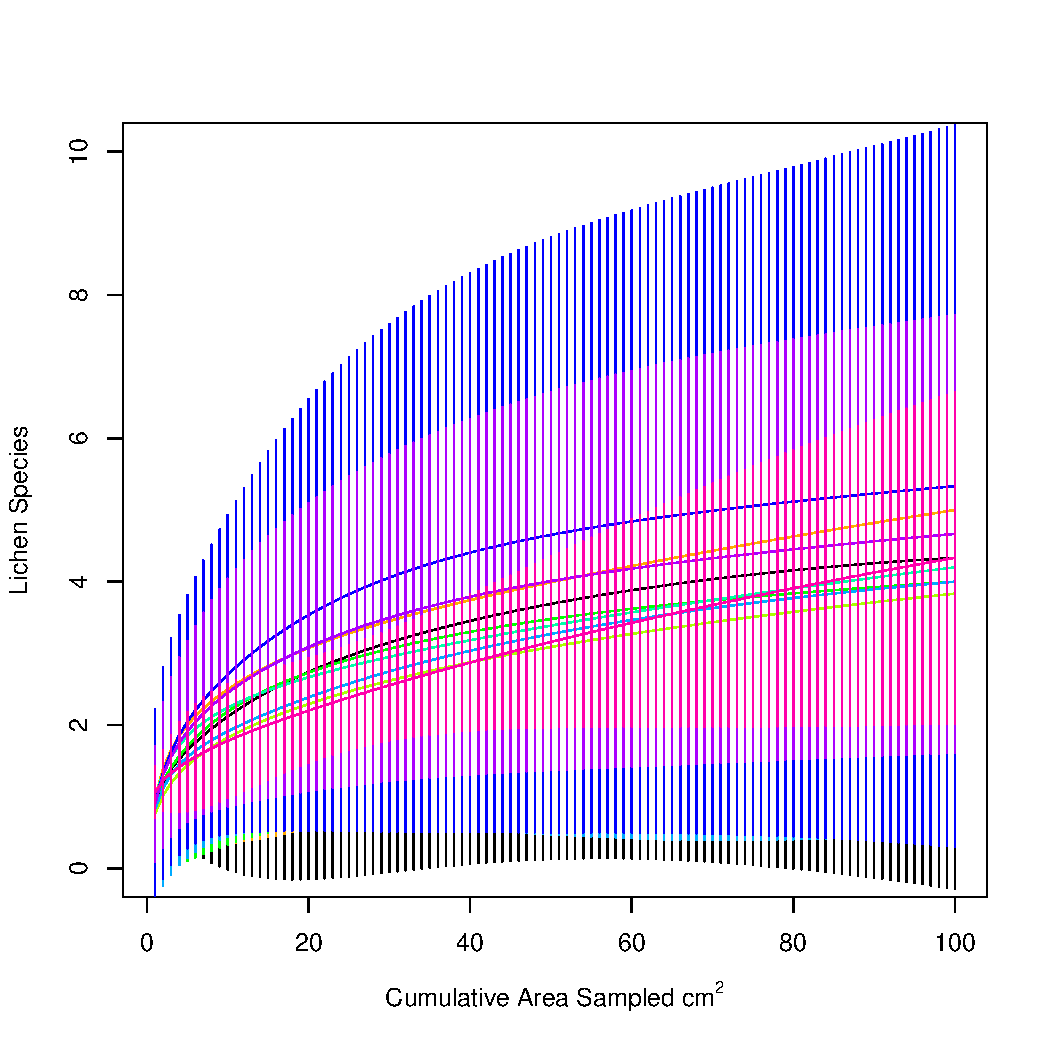
\includegraphics[width=\linewidth]{spac_geno.pdf}
\caption{Species area curve by genotype.}
\label{fig:spac_geno_app}
\end{figure*}


\begin{figure*}[ht]
\centering
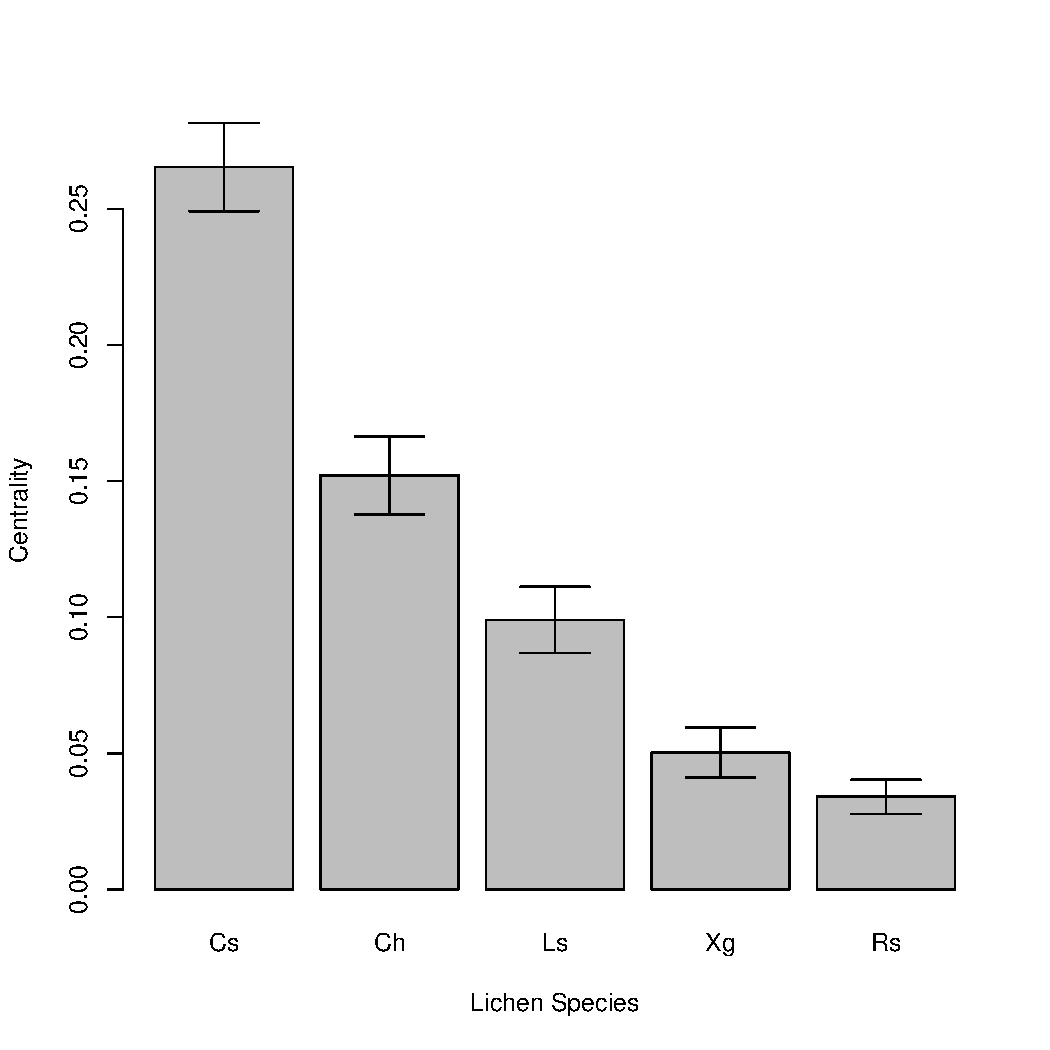
\includegraphics[width=\linewidth]{spp_cen.pdf}
\caption{}
\label{fig:spp_cen_app}
\end{figure*}

%% \begin{figure*}[ht]
%% \centering
%% 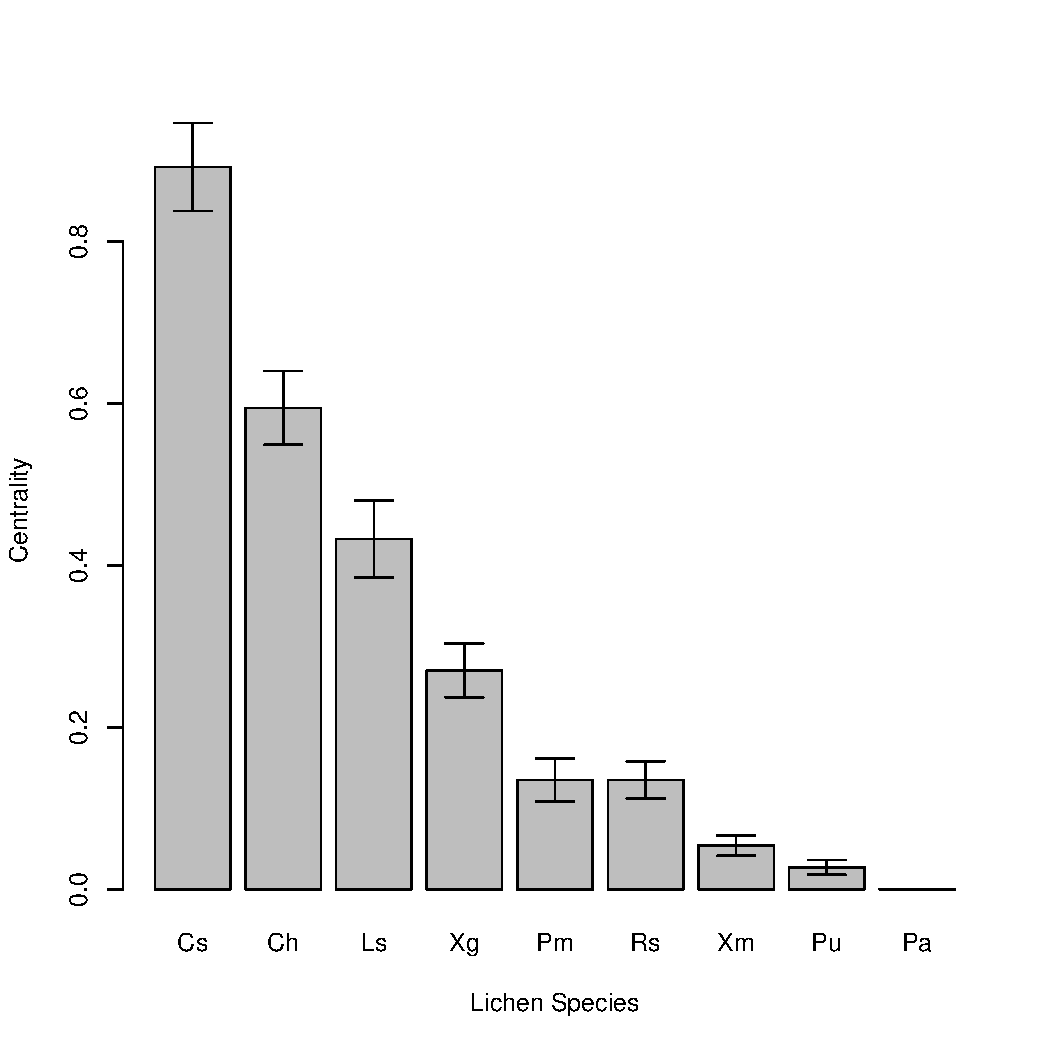
\includegraphics[width=\linewidth]{spp_cen_in.pdf}
%% \caption{}
%% \label{fig:spp_cen_in_app}
%% \end{figure*}

%% \begin{figure*}[ht]
%% \centering
%% 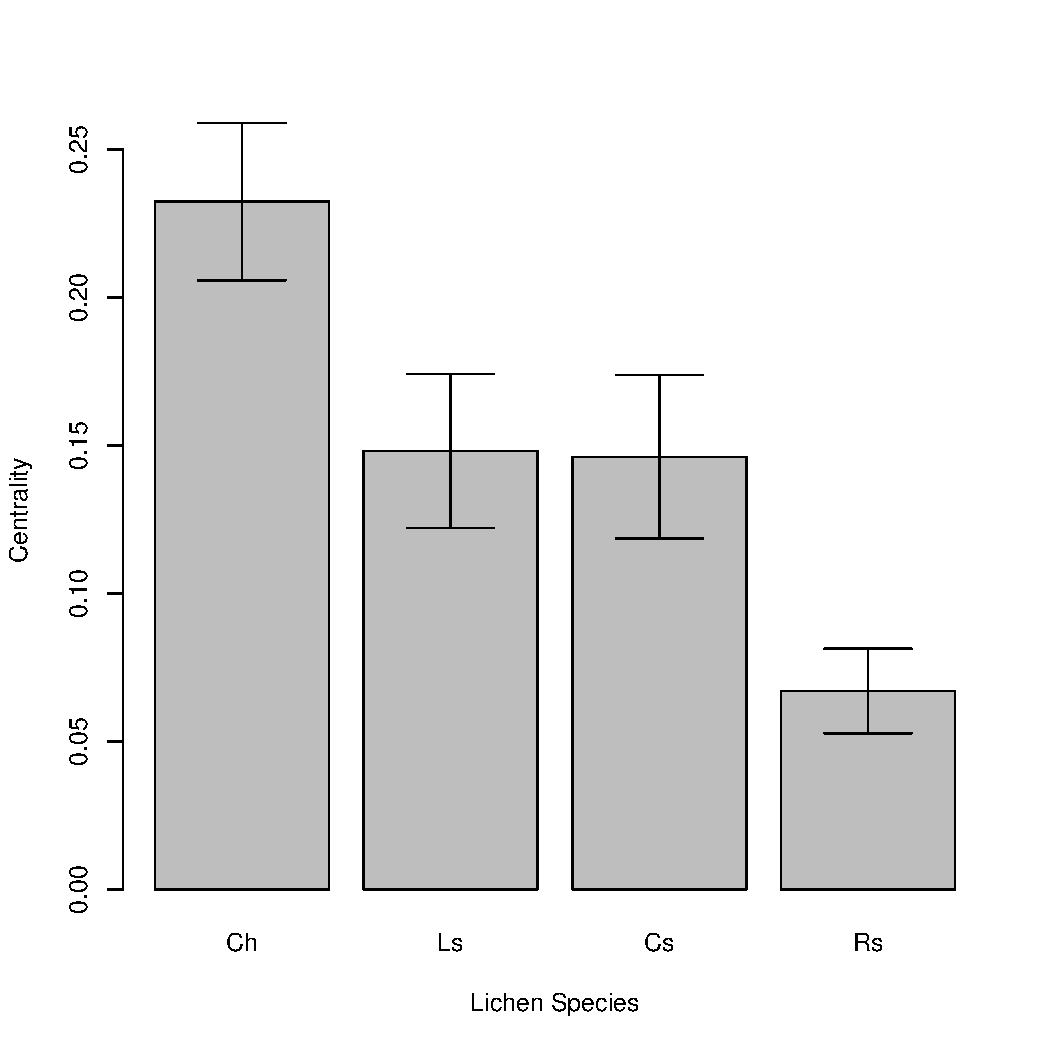
\includegraphics[width=\linewidth]{spp_cen_out.pdf}
%% \caption{}
%% \label{fig:spp_cen_out_app}
%% \end{figure*}

\end{document}

%% \subsection*{Supporting Information (SI)}

%% Authors should submit SI as a single separate PDF file, combining
%% all text, figures, tables, movie legends, and SI references.  PNAS
%% will publish SI uncomposed, as the authors have provided it.
%% Additional details can be found here:
%% \href{http://www.pnas.org/page/authors/journal-policies}{policy on
%% SI}.  For SI formatting instructions click
%% \href{https://www.pnascentral.org/cgi-bin/main.plex?form_type=display_auth_si_instructions}{here}.
%% The PNAS Overleaf SI template can be found
%% \href{https://www.overleaf.com/latex/templates/pnas-template-for-supplementary-information/wqfsfqwyjtsd}{here}.
%% Refer to the SI Appendix in the manuscript at an appropriate point
%% in the text. Number supporting figures and tables starting with S1,
%% S2, etc.

%% Authors who place detailed materials and methods in an SI Appendix
%% must provide sufficient detail in the main text methods to enable a
%% reader to follow the logic of the procedures and results and also
%% must reference the SI methods. If a paper is fundamentally a study
%% of a new method or technique, then the methods must be described
%% completely in the main text.

%% \subsubsection*{SI Datasets} 

%% Supply Excel (.xls), RTF, or PDF files. This file type will be
%% published in raw format and will not be edited or composed.

%% \subsubsection*{SI Movies}

%% Supply Audio Video Interleave (avi), Quicktime (mov), Windows Media
%% (wmv), animated GIF (gif), or MPEG files and submit a brief legend
%% for each movie in a Word or RTF file. All movies should be
%% submitted at the desired reproduction size and length. Movies
%% should be no more than 10 MB in size.


%% \subsubsection*{3D Figures}

%% Supply a composable U3D or PRC file so that it may be edited and
%% composed. Authors may submit a PDF file but please note it will be
%% published in raw format and will not be edited or composed.

